%%%%%% CMB-S4 Neutrinos Chapter  %%%%%%%%%%%%%%%%
 
\chapter{Neutrinos}
%\renewcommand*\thesection{\arabic{section}}


\def\beq{\begin{equation}}
\def\eeq{\end{equation}}

\def\bea{\begin{eqnarray}}
\def\eea{\end{eqnarray}}

\def\Neff{N_{\rm eff}}
\def\Nf{N_{\rm eff}}
\def\gs{g_{\star}}
\def\Mpl{M_{\rm pl}}
\newcommand{\nucl}[3]{ \ensuremath{ \phantom{\ensuremath{^{#1}_{#2}}} \llap{\ensuremath{^{#1}}} \llap{\ensuremath{_{\rule{0pt}{.75em}#2}}} \mbox{#3} } }


\def\gtrsim{\raise-.75ex\hbox{$\buildrel>\over\sim$}}
\def\lsim{\raise-.75ex\hbox{$\buildrel<\over\sim$}}
%%%%%%%%%%%%%%%%%%%%%%%%%%%%%%%%%%%%%%%%%%%%%%%%%%%%%%%%%%%
%%%%%%%%%%%%%%%%%%%%%%%%%%%%%%%%%%%%%%%%%%%%%%%%%%%%%%%%%%%
%%%%%%%%%%%%%%%%%%%%%%%%%%%%%%%%%%%%%%%%%%%%%%%%%%%%%%%%%%%
%%%%%%%%%%%%%%%%%%%%%%%%%%%%%%%%%%%%%%%%%%%%%%%%%%%%%%%%%%%

\begin{center}
{\small \it (send feedback on this chapter to \href{mailto:s4_neutrinos@cosmo.uchicago.edu}{s4\_neutrinos@cosmo.uchicago.edu})}
\end{center}

\begin{quotation}

Neutrinos are the last unexplored corner of the Standard Model of particle physics.  The 2015 Nobel Prize recognized the discovery of neutrino oscillations, which shows that they have mass. However, the overall scale of the masses and the full suite of mixing parameters are still not measured.  Cosmology offers a unique view of neutrinos; they were produced in large numbers in the hot temperatures of the early universe and left a distinctive imprint in the cosmic microwave background and on the large scale structure of the universe. Therefore, CMB-S4 and the large surveys DESI and LSST together will have the power to detect properties of neutrinos that supplement those probed by large terrestrial experiments such as DUNE and those searching for neutrino-less double beta decay.

Specifically, while DUNE and its predecessors are sensitive to the differences in the masses of the different types of neutrinos, CMB-S4  will probe the {\it sum} of all the neutrino masses, $\sum m_\nu$. The current lower limit is $\sum m_\nu c^2 > 60$ milli-eV. CMB-S4, in conjunction with other upcoming cosmic surveys, will measure this sum with high significance. Once determined, $\sum m_\nu$ will inform the prospects for future neutrino-less double beta decay experiments that aim to determine whether neutrinos are their own anti-particle. Finally, CMB-S4 is particularly sensitive to the possible existence of additional neutrinos that interact even more weakly than the standard three. These so-called {\it sterile} neutrinos are also being vigorously pursued with the Fermilab Short Baseline Program and at reactors around the world, so the combination of CMB-S4 with terrestrial probes adds up to a comprehensive assault on the three-neutrino paradigm. 


%ATL 7/14/16: original version

%Specifically, while DUNE and its predecessors are sensitive to the differences in the masses of the different types of neutrinos, CMB-S4  will probe the {\it sum} of all the neutrino masses, $\sum m_\nu$. The current lower limit is $\sum m_\nu c^2 > 60$ milli-eV. CMB-S4, likely by itself but certainly in conjunction with other cosmic surveys, will measure this sum with high significance. Once determined, $\sum m_\nu$ will inform the prospects for future neutrino-less double beta decay experiments that aim to determine whether neutrinos are their own anti=particle. Finally, CMB-S4 is particularly sensitive to the possible existence of additional neutrinos that interact even more weakly than the standard three. These so-called {\it sterile} neutrinos are also being vigorously pursued with the Fermilab Short Baseline Program and at reactors around the world, so the combination of CMB-S4 with terrestrial probes adds up to a comprehensive assault on the three-neutrino paradigm. 



%
%Although neutrinos contribute to the total matter density today, they are still sufficiently light that they free stream over cosmological distances.  As a result, neutrinos do not cluster the way conventional cold matter does, leading to a suppression of the fluctuations on small scales.  This suppression affects a number of cosmological observables from galaxies to the CMB. Gravitational lensing of the CMB is a particularly clean probe of matter distribution of the universe and, therefore, neutrino mass.  Through lensing, CMB Stage IV will be sensitive to the minimal possible neutrino mass at the 2-3$\sigma$ level and will robustly distinguish between the normal and inverted hierarchy.  Furthermore, measurements of the CMB are extremely sensitive to additional sterile neutrinos or other exotic physics in the neutrino sector and sensitivity to these possibilities is expected to improve by a factor of ten.

\end{quotation}

\section{Introduction}



Direct interactions between neutrinos and observable matter effectively ceased about one second after the end of inflation.  Nevertheless, the total energy density carried by neutrinos was comparable to other components through recent cosmological times.  As a result, the gravitational effect of the neutrinos is detectable both at the time of recombination and in the growth of structure at later times~\cite{Abazajian:2013oma}, leaving imprints in the temperature and polarization spectrum as well as in CMB lensing.

CMB-S4 can improve our understanding of neutrino physics in regimes of interest for both particle physics and neutrino cosmology.  Arguably the most important parameters of interest will be the sum of the neutrino masses ($\sum m_\nu$), the effective number of neutrino species ($\Neff$) and the helium fraction ($Y_p$).  These three parameters are highly constrained within the Standard Model of particle physics and will be precisely measured with a CMB-S4 experiment:
\begin{itemize}
\item $ \sum m_\nu \gtrsim \, 58$ meV is the lower bound guaranteed by observations of solar and atmospheric neutrino oscillations.  A CMB experiment with $\sigma(\sum m_\nu) < 20$ meV would be guaranteed a detection of at least 3$\sigma$.  At this level, one can detect the overall scale of the neutrino masses even for a normal ordered hierarchy.
\item $\Neff =  3.046$ and $Y_p \approx 0.2311 + 0.9502 \, \Omega_b h^2$ are predicted by standard neutrino decoupling and big bang nucleosynethesis (BBN).  $\Neff$ is a measure of the total radiation energy density at recombination while $Y_p$ is sensitive to the radiation density and the neutrino distribution at BBN. 
\end{itemize}
Current CMB data already provides a robust detection of the cosmic neutrino background at $\sim10 \sigma$.  A CMB-S4 experiment will provide an order of magnitude improvement in sensitivity in $\Neff$ that opens a new window back to the time of neutrino decoupling and beyond.  $\Neff$ and $Y_p$ are also sensitive to any additional light particles beyond the Standard Model, such as sterile neutrinos or axions.  The implications of these constraints will be explored in more detail in Chapter 4, where we will discuss the observational signatures and forecasts for future measurements of $\Neff$ and $Y_p$.  

Section~\ref{sec:neureview} will review neutrino cosmology and the motivation for studying neutrino masses with cosmological probes.  Section~\ref{sec:mnuobs} will discuss the various cosmological signatures of neutrino mass, emphasizing the CMB specifically.  We will forecast CMB Stage IV sensitivity to $\sum m_\nu$.  Section~\ref{sec:lab} will discuss the relationship between cosmological and lab based neutrino measurements, including a discussion of sterile neutrinos.  Section~\ref{sec:neuscenarios} will explore some possible scenarios for neutrino physics with CMB-S4 and neutrino experiments.

\section{ Review of Neutrino Cosmology}\label{sec:neureview}

Cosmological measurements of neutrinos depend on our detailed understanding of the cosmic history, starting with their decoupling at high temperatures ($T \lesssim 10$ MeV) through to their contribution to the growth of structure at late times.  In this Section we will give an overview of these epochs with an eye towards to the measurements of $\sum m_\nu$, $\Neff$ and $Y_p$ to be discussed in the next two chapters.  

\subsection{ Neutrino Physics Basics}

Measurements of $ \sum m_\nu $ by CMB-S4 will be interesting within the context of the broader neutrino experimental program. Neutrino flavor oscillations are described by a model where the neutrino flavor eigenstates are a mixture of massive neutrino eigenstates. The mixing is parameterized by the Pontecorvo-Maki-Nakagawa-Sakata (PMNS) matrix,
\[ \left( \begin{array}{c} \nu_e \\ \nu_{\mu} \\ \nu_{\tau} \\ \end{array} \right) = 
\left( \begin{array}{ccc} U_{e1} & U_{e2} & U_{e3} \\ U_{\mu1} & U_{\mu2} & U_{\mu3} \\ U_{\tau1} & U_{\tau2} & U_{\tau3} \\
\end{array} \right) \cdot
\left( \begin{array}{c} \nu_1 \\ \nu_2 \\ \nu_3 \\ \end{array} \right),
\]
where $\nu_{i}$, $i=1,2,3$ are the neutrino mass eigenstates. $U_{\rm PMNS}$ depends upon six real parameters: three mixing angles, $\theta_{12}$,  $\theta_{23}$, $\theta_{13}$ that
correspond to the three Euler rotations in a 3--dimensional space, and three phases, $\delta$, $\alpha_1$, $\alpha_2$. A suitable parametrization is
\[ U_{\rm PMNS}=
\left( \begin{array}{ccc} c_{12}c_{13} & s_{12}c_{13} & s_{13} e^{-i\delta} \\ 
-s_{12}c_{23} - c_{12}s_{13}s_{23} e^{i\delta} & c_{12}c_{23} - s_{12}s_{13}s_{23} e^{i\delta} & c_{13}s_{23} \\
s_{12}s_{23} - c_{12}s_{13}c_{23} e^{i\delta} & -c_{12}s_{23} - s_{12}s_{13}c_{23} e^{i\delta} & c_{13}c_{23} \\
\end{array} \right) \cdot
\left( \begin{array}{ccc} 1 & 0 & 0 \\ 0 & e^{i\alpha_1/2} & 0 \\ 0 & 0 & e^{i(\alpha_2/2)} \\ 
\end{array} \right)
\]
where $c_{ij} \equiv \cos\theta_{ij}$ and $s_{ij} \equiv \sin\theta_{ij}$. 
The phases $\delta$ ($\equiv \delta_{CP}$) and $\alpha_1$, $\alpha_2$ are Dirac--type and Majorana--type $CP$ violating phases, respectively.

Experiments have measured the three mixing angles of $U_{\rm PMNS}$ and the two mass splittings, $\Delta m^2_{21}$ (the ``solar'' mass splitting) and $\Delta m^2_{32}$ (the ``atmospheric'' mass splitting), but fundamental aspects of neutrino mass and mixing are yet to be settled. These include:
\begin{itemize}
\item measuring the absolute mass scale,
\item determining the mass ordering,
\item searching for Lepton number violation (i.e., determining whether neutrinos are Majorana particles) and
\item observing CP violation (measuring $\delta_{CP}$).
\end{itemize}
Exploring these goals is the focus of current and upcoming neutrino experiments. CMB-S4 will measure $ \sum m_\nu $ with sufficient sensitivity to be relevant to these open issues. Fig.~\ref{fig:neutrino-noose} shows the relationship between CMB-S4 measurements and other measures of neutrino mass and ordering and Fig.~\ref{fig:NLDBD} shows the connection between cosmological measurements of neutrino mass and neutrinoless doube beta decay experiments. 


\subsection{Thermal History of the Early Universe} \label{ThermalHistory}
In this section, we will give a sketch of the thermal history of the standard hot big bang universe when the temperature of the plasma was falling from about $10^{11}$~K to about $10^8$~K following Section 3.1 of \cite{Weinberg:2008zzc}.  For other reviews see \cite{Dolgov:2002wy,Agashe:2014kda}.  During this era, there are two events of particular interest: neutrinos decoupled from the rest of the plasma, and a short time later electrons and positrons annihilated, heating the photons relative to the neutrinos.  Our task is to follow how these events impact the evolution of the energy densities of the photons and neutrinos.

For massless particles described by the Fermi-Dirac or Bose-Einstein distributions, the energy density is given by
\beq
	\rho(T) =
	\Bigg\{\begin{array}{l c l}
        g\frac{\pi^2k_B^4}{30\hbar^3 c^3}T^4 &  &{\rm Boson}\\
       \frac{7}{8}g\frac{\pi^2k_B^4}{30\hbar^3 c^3} T^4 &  &{\rm Fermion}
        \end{array}
\eeq
where $g$ counts the number of distinct spin states.  The entropy density for massless particles is given by
\begin{equation}
	s(T) = \frac{4\rho(T)}{3T} \, .
\end{equation}
It is convenient to define a quantity $\gs$ which counts the spin states for all particles and antiparticles, with an additional factor $\frac{7}{8}$ for fermions.  With this definition, the total energy density and entropy density of the universe during radiation domination are given by
\bea
	\rho(T) &=& \gs\frac{\pi^2k_B^4}{30\hbar^3 c^3}T^4 \, , \nonumber \\
	s(T) &=& \frac{4}{3}\gs\frac{\pi^2k_B^4}{30\hbar^3 c^3}T^3 \, .
\eea
In an expanding universe, the first law of thermodynamics implies that for particles in equilibrium, the comoving entropy density is conserved
\begin{equation}
	a^3s(T) = \mathrm{const} \, .
\end{equation}
One straightforward consequence of this conservation is that for radiation in free expansion, the temperature evolves as the inverse of the scale factor
\begin{equation}
	T\propto \frac{1}{a} \, .
\end{equation}
Let us now apply this to the physics of the early universe.

At a temperature of $10^{11}$~K ($k_BT\sim10$~MeV), the universe was filled with photons, electrons and positrons, and neutrinos and antineutrinos of three species, all in thermal equilibrium with negligible chemical potential, along with a much smaller density of baryons and dark matter both of which are unimportant for the present discussion.  As the temperature of the plasma dropped below about $10^{10}$~K (about 1 second after the end of inflation), the rate of collisions between neutrinos and electrons and positrons could no longer keep up with the expansion rate of the universe, and neutrinos began to fall out of equilibrium and begin a free expansion.  Electrons and positrons remained in equilibrium with photons and their number densities fell with decreasing temperature, so that they were effectively gone by the time the temperature fell to $T \sim 10\,{\rm keV}$.  We will simplify the discussion by assuming that neutrinos decoupled instantaneously before electron-positron annihilation and comment below how a more detailed calculation modifies the results.  Non-zero neutrino masses can safely be neglected here as long as $m_\nu c^2\lesssim1$~keV which is guaranteed by current observational bounds.

From this point on, we will distinguish the temperature of neutrinos $T_\nu$ from that of the photons $T_\gamma$.  Before neutrino decoupling, frequent interactions kept neutrinos and photons in equilibrium, ensuring they had a common falling temperature.  After the universe became transparent to neutrinos, the neutrinos kept their relativistic Fermi-Dirac distribution with a temperature which fell as the inverse of the scale factor.  The photons, on the other hand, were heated by the annihilation of the electrons and positrons.  Comoving entropy conservation allows us to compute the relative temperatures at later times.

After neutrino decoupling, but before electron positron annihilation, the thermal plasma contained two spin states of photons, plus two spin states each of electrons and positrons, which means that during this period,
\begin{equation}
	g_{\star}^{\mathrm{before}} = 2 + \frac{7}{8}(2+2) = \frac{11}{2} \, .
\end{equation}
After electron positron annihilation, only the two spin states of photons remained, and so
\begin{equation}
	g_\star^{\mathrm{after}} = 2 \, .
\end{equation}
Since $T_\nu\propto a^{-1}$ during this period, we can express the condition of comoving entropy conservation as follows
\begin{equation}
	\frac{g_{\star}^{\mathrm{before}} \, T_{\gamma,\mathrm{before}}^3}{T_{\nu,\mathrm{before}}^3} = \frac{g_\star^{\mathrm{after}} \, T_{\gamma,\mathrm{after}}^3}{T_{\nu,\mathrm{after}}^3} \, .
\end{equation}
Using the fact that $T_{\gamma,\mathrm{before}} = T_{\nu,\mathrm{before}}$, we find as a result
\begin{equation}
	\frac{T_{\gamma,\mathrm{after}}}{T_{\nu,\mathrm{after}}} = \left(\frac{11}{4}\right)^{1/3} \, .
\end{equation}
We find that in the instantaneous neutrino decoupling limit, the annihilation of electrons and positrons raised the temperature of photons relative to that of neutrinos by a factor of $(11/4)^{1/3}\simeq1.401$.

After electron positron annihilation, assuming three species of light neutrinos and antineutrinos, each with one spin state, the radiation density of the universe is
\begin{equation}
	\rho_r = \frac{\pi^2k_B^4}{30\hbar^3 c^3}\left[2T_\gamma^4 + 3\frac{7}{8}T_\nu^4\right] = \frac{\pi^2k_B^4}{15\hbar^3 c^3}\left[1+3\,\frac{7}{8}\left(\frac{4}{11}\right)^{4/3}\right] T_\gamma^4 \, .
\end{equation}
It is conventional to define a quantity $\Nf$ which gives the radiation energy density in terms of the effective number of neutrino species as
\begin{equation}
	\rho_r = \frac{\pi^2k_B^4}{15\hbar^3 c^3}\left[1+\frac{7}{8}\left(\frac{4}{11}\right)^{4/3}\Nf\right] T_\gamma^4 \, .
\end{equation}
In the instantaneous neutrino decoupling approximation described above, we found $\Nf = 3$.  In the real universe, however, decoupling of neutrinos is not instantaneous, and the residual coupling of neutrinos at the time of electron positron annihilation increases $\Nf$ by a small amount in the Standard Model.

Unlike photon decoupling at temperature $T \sim 0.2$ eV, active neutrino decoupling at $T \sim 10 \, {\rm MeV} - 0.1 \, {\rm MeV}$ takes place over many tens of Hubble times, with the result that we expect distortions in the relic neutrino energy spectra relative to the thermal relativistic Fermi-Dirac distribution. Standard Model Boltzmann neutrino transport calculations show that these distortions change $\Neff$ at the percent level, with the current best estimate predicting $\Nf = 3.046$ \cite{Mangano:2005cc}.   This result is largely due to (1) the incomplete decoupling of neutrinos during electron-positron annihilation and (2) QED plasma effects.  While both effects have been calculated independently quite accurately, there is some theoretical uncertainty in this quantity at the level of about $10^{-3}$ due to the various numerical approximations that are made in the calculations when both effects are included simultaneously (see e.g.~\cite{Grohs:2015tfy} for discussion).  



\subsection{Neutrino Mass and Structure Formation}
\label{ssec:numasstheoryreview}
Cosmic background neutrinos are nearly as abundant in the universe as CMB photons. In the standard cosmological model, neutrinos ceased to scatter with other particles at temperatures $\sim 1 \, {\rm MeV}$. The relic neutrinos were relativistic at decoupling, but as the universe expanded and cooled the neutrino momenta redshifted as $p_\nu\propto 1/a$ and eventually the energy of most relic neutrinos came to be dominated by their rest mass, rather than their momentum. The energy density in nonrelativistic neutrinos therefore contributes to the matter budget of the universe today. The neutrinos, however, were relativistic for much of the history of the Universe so their gravitational clustering is qualitatively different from that of cold dark matter (CDM) particles. This difference can be used to distinguish the neutrino and cold dark matter contributions to the matter density \cite{Hu:1997mj, Lesgourgues:2006nd, Abazajian:2011dt}.  In this section, we review how neutrino mass affects the evolution of the neutrino energy density and the gravitational clustering of matter in the universe. 
 
As discussed more detail in the $\Neff$ section, cosmic background neutrinos have been detected indirectly through their contribution to the energy density in radiation in the early universe. The current CMB constraints from $\Neff$ are in excellent agreement with the Standard Model expectation of three species of neutrinos and antineutrinos each described very nearly by a relativistic thermal Fermi-Dirac distribution \cite{Ade:2015xua}. The distribution function for each species of neutrinos and antineutrinos (neglecting here the small non-thermal distortions discussed above) is given by
\beq
f_\nu(p) = \frac{1}{e^{a p/(k_BT_{\nu 0})} +1} \ ,
\eeq
where $T_{\nu 0} \approx 1.95K$ or $k_B T_{\nu 0} \approx 1.68 \times 10^{-4}\,{\rm eV}$ is the temperature today. Note that with Standard Model physics the spectral shape of the neutrino phase space distribution is preserved with the expansion so relic neutrinos have retained the relativistic Fermi-Dirac momentum distribution inherited from decoupling even as the individual neutrinos became non-relativistic. 

The neutrino energy density is given by
\beq
\rho_\nu = \sum_i \int\frac{d^3 {\bf p}}{(2\pi \hbar)^3} \frac{\sqrt{p^2 + m_{\nu i}^2}}{e^{ap/(k_BT_{\nu 0})} +1}
\eeq
where $m_{\nu i}$ are the three neutrino mass eigenstates.  For $T_{\nu}/a \gg m_{\nu i}$ the neutrino energies are dominated by their momenta and the total energy density behaves like radiation
\bea
\rho_{\nu}\Bigg|_{{\rm {\tiny early}}}  &\approx& \frac{7 \pi^2}{40}\frac{(k_B T_{\nu 0})^4}{\hbar^3 c^3}\frac{1}{a^4} \\
& \propto& a^{-4} \nonumber
\eea
While for $T_{\nu 0}/a \ll m_{\nu i}$ the energy density behaves like matter
\bea
\label{eq:rhonumassive}
\rho_{\nu} \Bigg|_{{\rm {\tiny late}}}  &\approx& \sum_i m_{\nu i} \bar{n}_\nu \\
&\propto& a^{-3} \nonumber
\eea
where $\bar{n}_\nu$ is the number of neutrinos and antineutrinos in each mass eigenstate
\beq
\bar{n}_\nu =\int\frac{d^3 {\bf p}}{(2\pi \hbar)^3} \frac{2}{e^{ap/(k_BT_{\nu 0})} +1} \approx \frac{113}{a^3}\,{\rm cm}^{-3}\,.
%&=&  \frac{6 \zeta(3)}{4\pi^2} \left(\frac{k_B T_\nu}{\hbar c}\right)^3\frac{1}{a^3}\\
\eeq

For a neutrino of mass $m_{\nu i}$ the transition between these two regimes ($T_\nu(a) \sim m_{\nu i}$) occurs at redshift $z_{\rm nr} \sim 300 (m_{\nu i}/0.05 {\rm eV})$. Using Eq.~(\ref{eq:rhonumassive}) the fractional energy density in neutrinos today can be written as
\beq
\Omega_\nu h^2 \approx \frac{\sum_i m_{\nu i}}{93\,{\rm eV}}\,.
\eeq
The individual masses of the neutrino states are unknown but neutrino oscillation data specifies the square of two mass splittings $\Delta m_{12}^2 = 7.54 \times 10^{-5}$~eV, $|\Delta m_{13}^2|\approx 2.4 \times 10^{-3}$~eV \cite{Agashe:2014kda}. These mass splittings, in combination with the neutrino number density, give a lower limit on the contribution of neutrinos to the cosmic energy budget
\beq
\Omega_\nu h^2 \,  \gtrsim \, 0.0006\,.
\eeq
At $z \ll z_{\rm nr}$ the matter density of the universe, which enters into the Hubble equation, is the sum of the CDM, baryon, and massive neutrino energy densities $\Omega_m = \Omega_c + \Omega_b + \Omega_\nu$. Whereas, at $z\gg z_{\rm nr}$ the matter density is solely made up of the baryon and CDM parts while neutrinos contribute to the radiation density. 

Neutrinos do not participate in gravitational collapse until late times when they have become nonrelativistic. Prior to this transition, the neutrinos {\em free-stream} out of gravitational wells, leaving the CDM and baryons behind  \cite{Bond:1983hb, Ma:1996za, Hu:1997vi, Hu:1997mj}. Primordial fluctuations in the neutrino density are therefore damped away on scales smaller than the horizon at $z_{\rm nr}$. In comoving units, this scale corresponds to a wave number
\beq
k_{\rm nr} \equiv a_{\rm nr} H(a_{\rm nr})/c \approx 0.003 \left(\frac{\Omega_m}{0.3}\frac{m_{\nu}}{0.05\, {\rm eV}}\right)^{1/2} h/{\rm Mpc}\,.
\eeq
Once the neutrinos are non-relativistic, their finite velocity dispersion still prevents them from clustering on scales smaller than the typical distance a neutrino travels in a Hubble time, $v_\nu /H(a)$ where $v_\nu \approx 3.15 T_{\nu 0}/(a m_\nu)$ the mean neutrino velocity. In analogy with the Jeans criterion for gravitational collapse, the neutrino free-streaming scale is defined by \cite{Bond:1983hb, Lesgourgues:2006nd}
\beq
k_{\rm fs}(a) \equiv \sqrt{\frac{3}{2}}\frac{aH(a)}{v_\nu(a)} \approx 0.04\, a^2 \sqrt{\Omega_m a^{-3} + \Omega_\Lambda}\left(\frac{m_\nu}{0.05 {\rm eV}}\right) h/{\rm Mpc}
\eeq
in comoving coordinates. 

On scales larger than $k_{\rm nr}$ (adiabatic) perturbations in the density of neutrinos, baryons, and CDM are coherent and can be described by a single perturbation to the total matter density $\delta_m= \delta \rho_m/\rho_m$. On smaller scales where the neutrino perturbations have decayed, only the perturbations to the CDM and baryons remain so that $\delta_{m} = \delta_{cb}\, (\Omega_{c} + \Omega_b)/\Omega_m $. The remaining CDM and baryon perturbations also grow more slowly because the neutrino energy density contributes to the expansion rate, but not to the source potentials. These two effects cause a suppression in the amplitude and the growth rate of matter perturbations wavenumbers $k > k_{\rm fs}$ relative to a universe with massless neutrinos (and also relative to density perturbations with $k<k_{\rm nr}$). The net change in the amplitude of perturbations with $k > k_{\rm nr}$ primarily depends on the fractional energy density in massive neutrinos (keeping $\Omega_c+\Omega_b$ fixed) but retains a small sensitivity to the individual neutrino masses through a dependence on $a_{\rm nr}$. A plot of the suppression in the matter power spectrum at small scales due to neutrino mass is shown in Figure \ref{fig:Psuppression}.


\begin{figure}[t]
\begin{center}
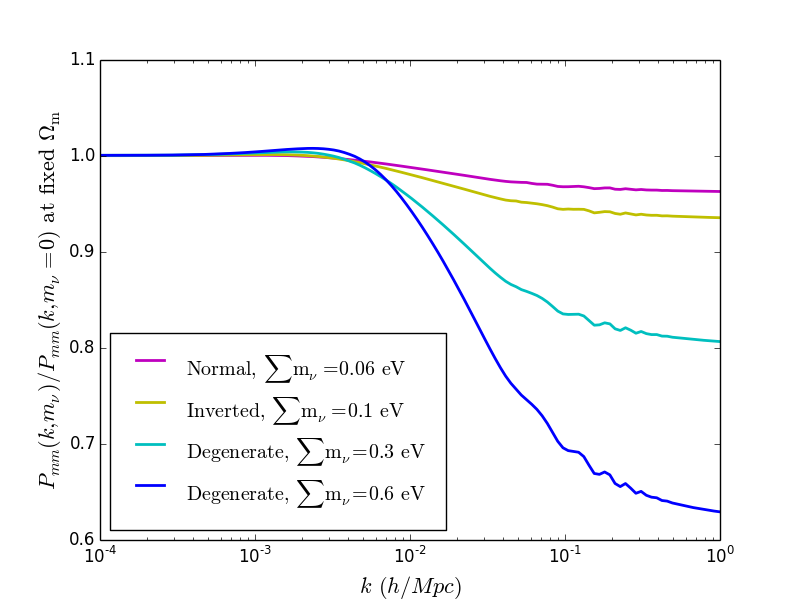
\includegraphics[width = 0.6\textwidth]{Neutrinos/Psuppression.png} 
\caption{ The suppression in the matter power spectrum due to massive neutrinos. Plotted is the ratio of the matter power spectrum for several neutrino mass hierarchies with $\sum m_\nu > 0$ to the matter power spectrum with $\sum m_\nu =0$ but the same value of $\Omega_m$. }
\label{fig:Psuppression}
\end{center}
\end{figure} 


An estimate of the effect of massive neutrinos on the growth of structure can be made by studying the evolution of matter perturbations in the two regimes $k\ll k_{\rm fs}$ and $k\gg k_{\rm fs}$.  In the synchronous gauge, linear perturbations to the matter density with wavenumbers $k \ll k_{\rm fs}$ evolve as
\beq
\label{eq:ddotdeltalarge}
\ddot{\delta}_m + 2 H(a) \dot\delta_m - \frac{3}{2}\Omega_mH_0^2 a^{-3}\delta_m = 0\quad {\rm for }\quad k \ll k_{\rm nr}
\eeq
which has solutions $\delta_m \propto a, \, a^{-\frac{3}{2}}$ during the matter dominated era. %On these scales, the evolution of matter perturbations just depends on $\Omega_m$, not on the fractional energy density in massive neutrinos. 

On scales where the neutrino perturbations have decayed, perturbations to matter density are just in the CDM and baryon components 
\beq
\delta_m(k\gg k_{\rm fs})\approx  (\delta\rho_c + \delta\rho_b)/\rho_m = (1-f_\nu)\delta_{cb}
\eeq 
where $f_\nu = \Omega_\nu/\Omega_m$ and $\delta_{cb} = (\delta\rho_c + \delta\rho_b)/(\rho_c + \rho_b)$, but the neutrino energy density still contributes to the Hubble friction. In this limit, linear perturbations to the  CDM and baryon density evolve as
\beq
\label{eq:ddotdeltasmall}
\ddot{\delta}_{m} + 2 H(a)\dot{\delta}_{m} - \frac{3}{2}\Omega_{cb}H_0^2 a^{-3} \delta_{m} =0\quad {\rm for}\quad  k \gg k_{\rm fs} 
\eeq
where $\Omega_{cb} = \Omega_c + \Omega_b$ and $\Omega_{cb} < \Omega_m$ for a cosmology with massive neutrinos. Equation (\ref{eq:ddotdeltasmall}) has the approximate solutions during the matter dominated era of $\delta_{cb} \propto a^{1-\frac{3}{5}f_\nu}, a^{-\frac{3}{2} + \frac{3}{5}f_\nu}$ for $f_\nu  \ll 1$. \

The matter dominated solutions give a simple estimate of the net effects of massive neutrinos on the amplitude of matter perturbations. For fixed $\Omega_c h^2$, the evolution of perturbations in a cosmology with $f_\nu \neq 0$ is the same as a cosmology with $f_\nu =0$. After $a_{\rm nr}$, the perturbations with $k\gg k_{\rm fs}$ grow more slowly (according to Eq.~(\ref{eq:ddotdeltasmall}), the growing mode solution grows as  $\propto a^{1-\frac{3}{5}f_\nu}$) than those with $k\ll k_{\rm fs}$ (according to Eq.~(\ref{eq:ddotdeltalarge}), $\propto a$).  At scale-factor $a$ during the matter dominated era, the total difference in growth or perturbations with $k\gg k_{\rm fs}$ is roughly
\beq
\frac{\delta_{cb}(k \gg k_{\rm fs}, a | f_\nu)}{\delta_{cb}(k \gg k_{\rm fs}, a | f_\nu=0)} \sim \left(\frac{a}{a_{\rm nr}}\right)^{-\frac{3}{5}f_\nu}\,.
\eeq
The resulting difference in the amplitude of the matter power spectra is then 
\beq
\frac{P_{mm}(k \gg k_{\rm fs}, a  |f_\nu)}{P_{mm}(k \gg k_{\rm fs}, a |f_\nu =0)}\sim (1-2f_\nu)\frac{P_{cc}(k \gg k_{\rm fs} , a |f_\nu)}{P_{cc}(k \gg k_{\rm fs}, a |f_\nu =0)}\sim \left(1-2f_\nu -\frac{6}{5}f_\nu\ln\left(a/a_{\rm nr}\right)\right)\,.
\eeq
On the other hand, the evolution of the large scale modes is identical,
\beq
\frac{P_{mm}(k \ll k_{\rm fs}, a  |f_\nu)}{P_{mm}(k \ll k_{\rm fs}, a |f_\nu =0)}=1\,.
\eeq
where $P_{mm}$ is the power spectrum of the total matter fluctuations (CDM, neutrino, and baryon) and $P_{cc}$ is the power spectrum of just the CDM and baryons.  The above expression overestimates the effect of neutrino mass by assuming the transition from relativistic to non-relativistic is instantaneous. It also ignores the effects of the cosmological constant at late times. Using the true evolution of $\delta_{cb}$ through $a_{\rm nr}$ and allowing for the cosmological constant gives 
\beq
\frac{P_{mm}(k \gg k_{\rm fs} |f_\nu)}{P_{mm}(k \gg k_{\rm fs} |f_\nu =0)} \approx 1- 6 f_\nu
\eeq
at $a=1$. Note that this expression assumes fixed $\Omega_ch^2$, $\Omega_bh^2$ so that matter-radiation equality is not changed by neutrino mass and that and $\Omega_\Lambda = 1-\Omega_m$ is fixed by adjusting $h$ so that the onset of cosmological constant domination is also unchanged. Alternatively, assuming fixed $\Omega_m$ and decreasing $\Omega_{cb}$ to account for $\Omega_\nu$ makes matter-radiation equality, which occurs while the neutrinos are relativistic, slightly later so that the suppression is increased to
\beq
\frac{P_{mm}(k \gg k_{\rm fs} |f_\nu)}{P_{mm}(k \gg k_{\rm fs} |f_\nu =0)} \approx (1-8f_\nu)\,.
\eeq

\section{Cosmological Measurements of Neutrino Mass} \label{sec:mnuobs}


As explained in the previous section,  the signature of massive neutrinos manifests through
the energy density $\Omega_\nu$, which is related to the mass through
\beq
\Omega_\nu h^2 \simeq \, \frac{\sum m_\nu}{93 \, {\rm eV}} \, \gtrsim  \, 0.0006  \ .
\eeq
The lower limit on $\Omega_\nu h^2$ is a reflection of the lower limit on the sum of the masses, $\sum m_\nu \, \gtrsim  \, 58 \, {\rm meV}$, that is determined from neutrino oscillation experiments \cite{Agashe:2014kda}.  This sets a clear observational target for future observations.

Any probe of $P_{mm}$ late times is, in principle, sensitive to the sum of the neutrino masses.  The question we will be most interested in is whether a given probe is sensitive to the lower limit, $\sum m_\nu = 58 \, {\rm meV}$ (or $\Omega_\nu h^2 = 0.0006$) under realistic circumstances.  In this subsection, we will discuss the two methods through which CMB Stage IV can directly constrain the neutrino mass, CMB lensing and SZ cluster abundances.  We will also compare these observables to other cosmological probes of the neutrino mass from upcoming large scale structure surveys such as DESI and LSST.


\subsection{CMB Lensing}\label{sec:neulens}

Likely the cleanest probe of the neutrino mass in the CMB is through gravitational lensing~\cite{Kaplinghat:2003bh}, which directly measures the matter distribution along the line of sight.  To be concrete, in the Limber approximation, the lensing power spectrum is given by
\bea
\label{eq:CellPhiPhi}
C_\ell^{\phi \phi} &=& \frac{8\pi^2}{\ell^2} \int^{\chi_\star}_0 \chi d\chi P_\Psi(\ell /\chi ; \eta_0 - \chi)  \frac{(\chi_\star -\chi)^2}{\chi_\star \chi} \\
P_\Psi (k;\eta)&=& \frac{9 \Omega_m^2 (\eta) H^4(\eta)}{8 \pi^2} \frac{P_{mm}(k;\eta)}{k}
\eea
where $\chi$ ($\chi_\star$) is the co-moving distance (to the last scattering surface) and $\eta$ ($\eta_0$) is conformal time (today).   More details regarding CMB lensing, including current and future measurements, will be discussed in Chapter **.

For the purposes of the neutrino mass measurement, the advantage of lensing over other probes is that it is largely free of astrophysical uncertainties.  As we see from the lensing power spectrum, we are directly sensitive to the matter power spectrum (rather than a biased tracer) and the relevant scales are in the linear regime where modeling should be reliable.

The primary challenges for the lensing measurement are degeneracies with other cosmological parameters.  The two primary degeneracies in $\Lambda$CDM are
\begin{itemize}
\item Optical depth, $\tau$: The suppression of small scale power at low redshift requires a reliable measurement of the amplitude of the power spectrum at high redshift.  In principle, this is measured by the primary CMB anisotropies, but the overall normalization is degenerate with $\tau$ for $\ell \gtrsim 20$.  A precise measurement of $\tau$ is therefore crucial to calibrate the suppression at low redshifts.  Such a measurement will likely come from $\ell \lesssim 20$ polarization data from CMB-S4 and/or other CMB experiments.  It should be emphasized that Stage IV sensitivity is not needed for the measurement of $\tau$ and such a measurement could be performed by Planck or a Stage III experiment.


\item $\Omega_m h^2$ : The amount of lensing is controlled by the total amount of matter.  Therefore, we can compensate for a suppression from neutrinos by increasing the matter power spectrum.  This degeneracy will be broken by DESI BAO measurements of the expansion history.
\end{itemize}
In addition to degeneracies in $\Lambda$CDM there can be degeneracies with possible extensions.  Most notably:
\begin{itemize}
\item $\Neff$: The density of neutrinos after they become non-relativistic is given by $\rho_\nu \simeq m_\nu n_\nu$ where $n_\nu$ is the number density.  Therefore, we only measure the mass if we know the number density to sufficient accuracy.  Fortunately, as we will discuss in the next chapter, measurements of the neutrino energy density from the primary CMB will be sufficiently accurate as to make this degeneracy insignificant under plausible assumptions.
\end{itemize}
In principle, measurement of the free streaming scale directly in the matter power spectrum would separate the neutrino mass from most other physical quantities.  Unfortunately, given current limits on the neutrino mass, the change to the shape of the lensing potential power spectrum is not expected to drive future constraints.  

{\it Status of current observations} -- Planck has provided a strong constraint of $\sum m_\nu < 0.194$ eV when combining both temperature and polarization data with the CMB lensing power spectrum and external data.  A weaker constraint of $\sum m_\nu < 0.492$ eV can be derived using only the temperature and polarization data.  This constraint arises through the effect of massive neutrinos on the primordial TT and EE power spectra.  For sufficiently large masses, the neutrinos do not behave as radiation around the time of recombination which impacts the damping tail and locations of the acoustic peaks.  Improvements in the limits on the sum of the neutrino masses will be driven primarily by lensing given that current limits imply that the neutrinos are effectively massless from the point of view of the primary CMB anisotropies.  External data (BAO) will continue to be important in breaking the degeneracy with $\Omega_m$.  

\subsection{Other Cosmological Probes}

\subsubsection{Galaxy Cluster Abundance}
Galaxy clusters form from rare high peaks in the matter density field. A galaxy cluster of mass $M$ forms from a region of size $R\sim \left(M/(4/3\pi \bar\rho_m)\right)^{1/3}$, which is smaller than the neutrino free streaming scale for even the most massive galaxy clusters so long as $m_{\nu i} \lsim 0.1$eV. The neutrino free-streaming therefore slows the growth of structure on cluster scales, suppressing the abundance of galaxy clusters. 


The number density of clusters with mass $M$ can be expressed by (e.g. \cite{Tinker:2008ff,Bhattacharya:2010wy}), 
\beq
\label{eq:clmfcn}
\frac{dn}{dM}(M,z) = \frac{\rho}{M}\frac{d\ln \sigma^{-1}}{dM} f(\sigma, z)
\eeq
where $\sigma = \sigma(M,z)$ is the variance of linear perturbations in CDM and baryons on mass scale $M$ given by
\beq
\label{eq:sigmaM}
\sigma^2(M, z) = \int \frac{dk}{k} \frac{4\pi}{(2\pi)^3} P_{cc}(k, z) |W(kR)|^2
\eeq
where $R = (3M/(4\pi \rho_{cb}))^{1/3}$, $P_{cc}(k)$ is the power spectrum of CDM and baryons, and $W(kR) = 3(\sin(kR)/(kR)^3 - \cos(kR)/(kR)^2)$ is a top-hat window function \cite{Costanzi:2013bha,LoVerde:2014rxa}. The cluster abundance is extremely sensitive to $\sigma(M, z)$, and therefore $\sum m_\nu$ via the suppression in $P_{cc}$ discussed in \S\ref{ssec:numasstheoryreview}.

Current constraints on neutrino mass from cluster abundance, in combination with the primary CMB and BAO, are $\sum m_\nu \lsim 0.2$--$0.3$\,eV at $95\%$ confidence \cite{Hasselfield:2013wf,Mantz:2014paa,Ade:2015fva,deHaan:2016qvy}. To date, the contraints have been driven by the difference between (or consistency of) the matter power spectrum amplitude measured at late times, from clusters, and at early times, from the CMB. An additional signal is present internally to the cluster data, namely the time-dependent influence of massive neutrinos on cluster growth through Eqs.~\ref{eq:clmfcn} and \ref{eq:sigmaM}, which can potentially provide tighter constraints \cite{Wang:2005vr}.


Making these measurements of cluster abundance and growth require cluster surveys with well understood selection functions extending to high redshift ($z\sim2$). Galaxy clusters can be identified from CMB data via the thermal Sunyaev-Zel'dovich (tSZ) effect, the frequency shift of CMB photons that have scattered off of electrons in the hot, intra-cluster gas.  CMB-S4 is projected to detect a nearly mass-limited sample of $\mathcal{O}(100,000)$ galaxy clusters.

Given such a survey, the primary systematic limitation on cluster measurements of the neutrino mass, through either of the approaches above, is cluster mass estimation. This can be usefully broken into two problems: that of absolute mass calibration, i.e.\ our ability to measure cluster masses without bias on average, and relative mass calibration. The former is required for accurate inference of the power spectrum amplitude, while the latter significantly boosts cosmological constraints by providing more precise measurements of the shape and evolution of the mass function. Precise relative mass information can be provided by X-ray observations of the intracluster medium using existing ({\it Chandra}, XMM-{\it Newton}) and future (eROSITA, ATHENA) facilities; for the most massive SZ-selected clusters, found in existing CMB surveys, this work is already well advanced \cite{deHaan:2016qvy, Andersson:2010vy}. 

For absolute mass calibration, the most robust technique currently is galaxy-cluster weak lensing, which (with sufficient attention to detail) can provide unbiased results \cite{Corless:2009hi,Becker:2010xj}. At redshifts $z\lsim1$, residual systematic uncertainties in the lensing mass calibration are at the $\sim7\%$ level currently \cite{Applegate:2012kr}, and reducing these systematics further is the focus of significant effort in preparation for LSST and other Stage 4 data sets, with 1--2\% mass calibration at low redshifts seen as an achievable goal \cite{Abate:2012za}. Lensing of the CMB by clusters has also been measured \cite{Madhavacheril:2014slf,Baxter:2014frs}, and provides an additional route to absolute mass calibration. CMB-cluster lensing is particularly well suited to calibrating clusters at high redshifts ($z\gtrsim1$) where ground-based galaxy-cluster lensing becomes less efficient. CMB data with sufficient resolution and depth (especially in polarization) can potentially provide a percent-level mass calibration at these redshifts~\cite{Hu:2007bt}, comparable to galaxy-cluster lensing at lower redshifts.

As with dark energy studies, there are strong synergies between the SZ cluster catalog and CMB-cluster lensing information that CMB-S4 can provide when combined with external cluster surveys. The complementarity is particularly strong with LSST, which will provide highly mass-complete cluster catalogs out to redshifts $\sim1.2$ and competitive lensing measurements for clusters at $z\lsim 1$. In contrast, CMB-S4 will cleanly select the most massive clusters at all redshifts of interest for cluster cosmology through the SZ effect, and CMB lensing data can provide the key mass calibration for clusters at the highest redshifts detected by either survey. The latter especially provides the longest possible lever arm for detecting the time-dependent impact of neutrino mass on the growth of clusters. Because their systematic uncertainties are not identical, the combination of galaxy-cluster and CMB-cluster lensing information can straightforwardly produce tighter constraints on the power spectrum amplitude than either alone. The prospects for Stage 4 cluster data sets to definitively detect the neutrino mass are thus strong \cite{Mantz:2014paa,Wang:2005vr}.




\subsubsection{CMB Measurements in Context with Other Datasets}
Current and future large-scale structure surveys, such as BOSS, DES, DESI, LSST, Euclid, and WFIRST, provide maps of the distribution of mass and galaxies in the late universe\footnote{While these surveys measure structure by a variety of means (the distribution of galaxies or quasars, weak gravitational lensing, and the Lyman-$\alpha$ forest, for example) we refer to all of them as galaxy surveys.}. Large-scale structure datasets are primarily sensitive to the neutrino mass scale via two means: (i) the suppression of the matter power spectrum, which can be inferred from weak gravitational lensing \cite{Tereno:2008mm}, fluctuations in the number of galaxies \cite{Xia:2012na, Cuesta:2015iho}, or fluctuations in the opacity of intervening gas \cite{Palanque-Delabrouille:2014jca}, for example, and (ii) the change in the growth rate of matter perturbations which is inferred from redshift-space distortions (RSD)\cite{Beutler:2014yhv}. The first effect, the suppression in the matter power spectrum, is the same effect tested by CMB lensing.  The primary qualitative difference between information from galaxy surveys and the CMB is that galaxy surveys measure structure at multiple epochs in cosmic history whereas the CMB provides a map of the integrated mass distribution out to the surface of last scattering. The LSS information content in galaxy surveys is therefore greater than the CMB, but interpreting the data can be considerably more complex because the structure measured in galaxy surveys is typically more nonlinear and the relationship between the galaxy and mass distribution is less well-understood (in fact, massive neutrinos can make this even more complicated \cite{LoVerde:2014pxa}). Importantly, many of the observational and astrophysical systematics in the CMB and galaxy surveys are different, so the two approaches to measuring the neutrino mass scale are complementary. A summary of the forecasted constraints on $\sum m_\nu$ from galaxy surveys is given in Table \ref{table:numassLSS} \cite{Font-Ribera:2013rwa}. 
\begin{table}[t!]
\begin{center}
\begin{tabular}{|c|c|} 
\hline
    				  Datasets 			& $\sigma_{\sum m_\nu}$(eV) \\
				  \hline
Planck + DES lensing and galaxy clustering 		& 			0.041		\\
\hline
Planck + DESI Lyman-$\alpha$ Forest + BAO           &			0.098		\\
\hline
Planck + DESI Galaxy Power spectrum + BAO         &			0.024		\\
\hline
Planck + LSST Lensing and Galaxy Clustering         &   0.02					\\
\hline
\end{tabular}
\caption{Forecasted constraints on neutrino mass from future galaxy surveys in combination with Planck CMB from \cite{Font-Ribera:2013rwa}.  These forecasts assume Planck Blue Book priors for $\tau$, which is a stronger assumption than we apply to our forecasting.  See related discussion in Section~\ref{sec:nuforecasts}. }
\label{table:numassLSS}
\end{center}
\end{table}

There are a number synergistic opportunities between CMB-S4 and external cosmological datasets. For instance, the large-scale structure measured by galaxy surveys gravitationally lenses the CMB so there is a physical correlation between the CMB lensing convergence and e.g. the galaxy distribution or weak lensing shear maps inferred from galaxy surveys. Constraints on neutrino mass can therefore be tightened by cross-correlating maps of structure from galaxy surveys with the lensing information from the CMB (e.g.\ \cite{Takeuchi:2013gpa, Pearson:2013iha}). Or, the CMB can be cross-correlated with galaxy survey data to constrain neutrino mass via the mean pair-wise momentum of galaxy clusters \cite{Mueller:2014dba}. Additionally, CMB-S4 data indirectly aid measurements of neutrino mass from galaxy surveys because the CMB data can be used to calibrate systematics in weak lensing shear data \cite{Das:2013aia}. 





\subsection{Forecasts}\label{sec:nuforecasts}



\begin{figure}[h!]
\begin{center}
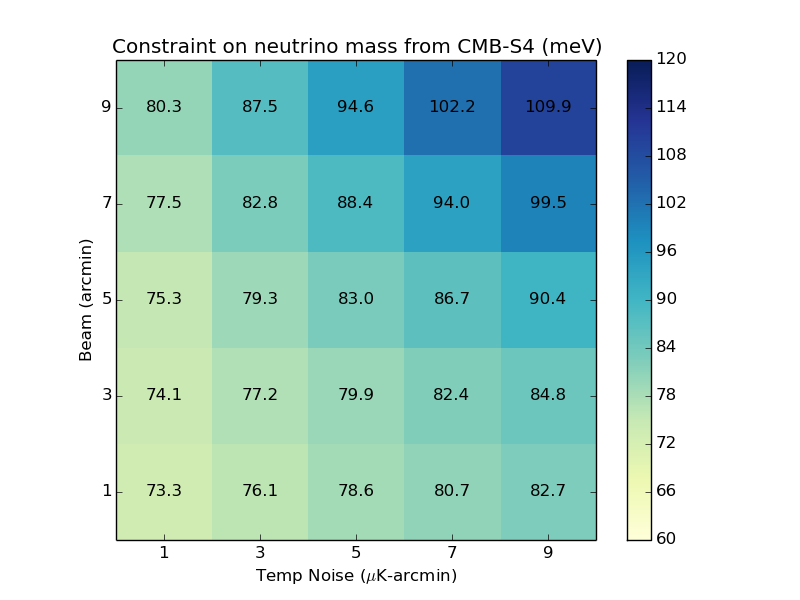
\includegraphics[scale=0.4]{Neutrinos/S4_BeamVsNoise.png}
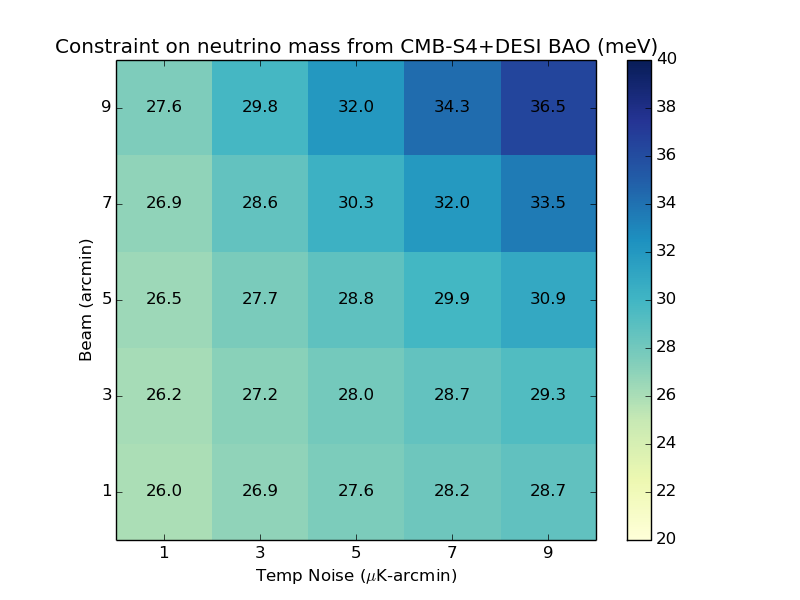
\includegraphics[scale=0.4]{Neutrinos/S4+DESI_BeamVsNoise.png}  
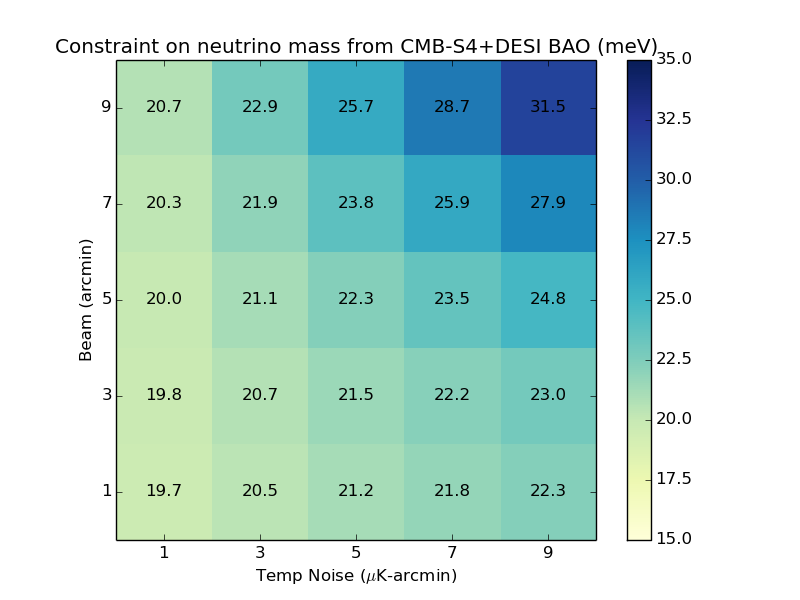
\includegraphics[scale=0.4]{Neutrinos/S4+DESI_BeamVsNoise_tauprior.png}

\caption{ Forecasts for $\sigma(\sum m_\nu)$ assuming $\Lambda$CDM + $\sum m_\nu$.  Both figures vary beam size in arcmin and effective detector noise in $\mu$K-arcmin. {\it Left:} CMB Stage IV alone with an external prior on $\tau = 0.06 \pm 0.01$. {\it Right: } CMB Stage IV with DESI BAO  with an external prior on $\tau = 0.06 \pm 0.01$.  {\it Bottom:} Forecasts assuming a prior $\tau = 0.06 \pm 0.006$, corresponding to the Planck Blue Book expected sensitivity.}
\label{fig:mnuforecast}
\end{center}
\end{figure} 

Target thresholds for $\sigma(\sum m_\nu)$ are $20$ meV and $30$ meV, corresponding to 3$\sigma$ and 2$\sigma$ detections of the minimum value for the normal hierarchy, $\sum m_\nu \sim 58$ meV.  Our goal is to explore the degree to which CMB Stage IV can reach these targets with realistic forecasts.  

The most concrete constrains on $\sum m_\nu$ from the CMB are derived from the CMB lensing power spectrum, as seen in Equation~(\ref{eq:CellPhiPhi}).  Our sensitivity to $\sum m_\nu$ is the limited by the error in the reconstruction of $\phi$ from the $T$ or $E/B$ maps.  The noise for the lensing reconstruction is discussed in detail in Section~\ref{sec:lensing_intro} and the noise curves for both the $TT$- and $EB$-estimators are show in Figure~\ref{n0s_s4}.  There are many reasons to prefer the $EB$-estimator which motivates a sensitivity $< 5 \, \mu K$-arcmin.  


 

Forecasts for CMB Stage IV with and without DESI BAO are shown in Figure~\ref{fig:mnuforecast}, following the methodology outlined in Section~\ref{sec:Forecasting}.  As we explained in Section~\ref{sec:neulens}, the main signature neutrino mass in CMB lensing is degenerate with both $\tau$ and $\Omega_m h^2$.  The sensitivity is therefore strongly dependent on the constraints on these parameters both internally and with external data.  We can see the effect of the measurement of $\Omega_m h^2$ by comparing the results with and without DESI BAO.  In particular, we note that the constraints improve by a factor or three by including DESI.

Including DESI BAO, the most significant limitation to measuring $\sum m_\nu$ is measurement of $\tau$.  We have assumed that $\ell \geq 30$ and therefore we do not constrain $\tau$ directly.  Under such circumstances, one is limited by the $\tau$-measurements by other experiments.  

By far the most conservative assumption is that the current Planck measurement is the best measurement that will be available, roughly corresponding to an external prior of $\tau = 0.06 \pm 0.01$.  We see in Figure~\ref{fig:mnuforecast}  that the current measurement is sufficient to reach $\sigma(\sum m_\nu) < 30$ meV for a wide range of experimental configurations.  On the other hand, we also note that there is little improvement with decreased noise or beamsize as we saturate at $\sigma(\sum m_\nu) \sim 26$ meV,  even if we increase $f_{\rm sky} >0.4$.  Of course, the reason is that we are limited by the $\tau$-degeneracy.


\begin{figure}[h!]
\begin{center}
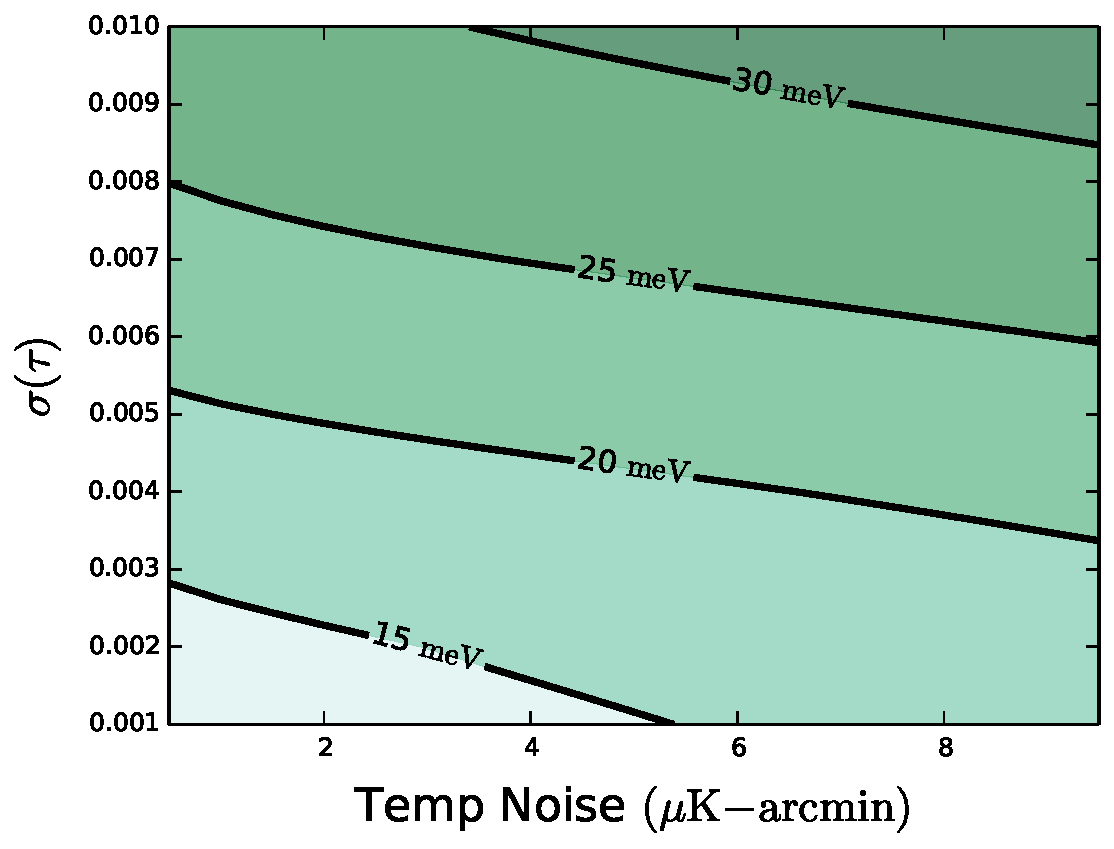
\includegraphics[scale=0.6]{Neutrinos/Mnu_tauprior.pdf}

\caption{ Forecasts for $\sigma(\sum m_\nu)$ assuming $\Lambda$CDM + $\sum m_\nu$ using CMB Stage IV and DESI BAO.  We vary sensitivity in $\mu$K-arcmin and $\tau$-priors, $\tau = 0.06 \pm \sigma(\tau)$ with the contours showing 1$\sigma$ errors for $\sum m_\nu$.  The white and blue dashed lines correspond to the low-$\ell$ cosmic variance limit and Planck Blue Book values respectively. }
\label{fig:mnu_tau}
\end{center}
\end{figure} 

In order to reach the 3$\sigma$ target, $\sigma(\sum m_\nu) < 20$ meV, one needs to assume a better measurement of $\tau$ will be available in the future.  One somewhat mild assumption is that Planck will reach a its designed reach in sensitivity.  As shown in bottom panel of Figure~\ref{fig:mnuforecast}, a measurement at the level of $\sigma(\tau) = 0.006$, we can reach $\sigma(\sum m_\nu) \sim 20$ for a variety of plausible configurations.  However, as before, we see that there are only moderate improvements coming from lower noise or smaller beams.  We see a similar limitation that applies to other cosmological probes, as seen in Table~\ref{table:numassLSS}, which also saturate at a similar sensitivity.

More generally, because we are limited only by degeneracies, we should also allow measurements of $\tau$ and $H_0$ that occur during or after the data has been collected.  Any such measurement should provide significant improvements in sensitivity the neutrino mass. Allowing for such possibilities, we consider the impact of stronger priors on $\tau$.  The right panel of of Figure~\ref{fig:mnu_tau} shows the 1$\sigma$ errors on $\sum m_\nu$ for varying $\tau$-priors.  We see that to reach a 4$\sigma$ detection of the minimum neutrino mass, $\sigma(\sum m_\nu) \sim 15$ meV, is possible for $\sigma(\tau) > 0.002$ for temperature noise $< 2 \, \mu$K-arcmin.  The value of $\sigma(\tau) \sim 0.002$ is the approximate cosmic variance limit achievable from the CMB, which would require a stage 3-4 experiment to reach $\ell_{\rm min} \sim 10$~\cite{Allison:2015qca} (although improvements in $\tau$/$\sum m_\nu$ require only $\ell_{\rm min} \lesssim 20$).













%%%%%%%%%%%%%%%%%%%%%%%%%%%%%%%%%%%%%%%%%
%%%%%% Placeholder for Neelima's systematics discussion %%%%%%%%%%
%%%%%%%%%%%%%%%%%%%%%%%%%%%%%%%%%%%%%%%%%




\section{Relation to Lab Experiments}\label{sec:lab}


\subsection{Determining the neutrino mass scale}
As discussed above, CMB-S4 will make a cosmological measurement of $\sum m_\nu$ and thus the neutrino mass scale. This approach complements terrestrial measurements of the neutrino mass using radioactive decay. These kinematic measurements of neutrino mass focus on one of two processes, beta-decay or electron-capture, where the decay spectra near the decay endpoint is particularly sensitive to the mass of the neutrino (see Fig.~\ref{fig:kinematic_mass}).
%to measure the kinematic impact measurements from tritium decay~\cite{Drexlin:2013lha} and neutrino-less double beta decay~\cite{}.

\begin{figure}[h!]
\centering
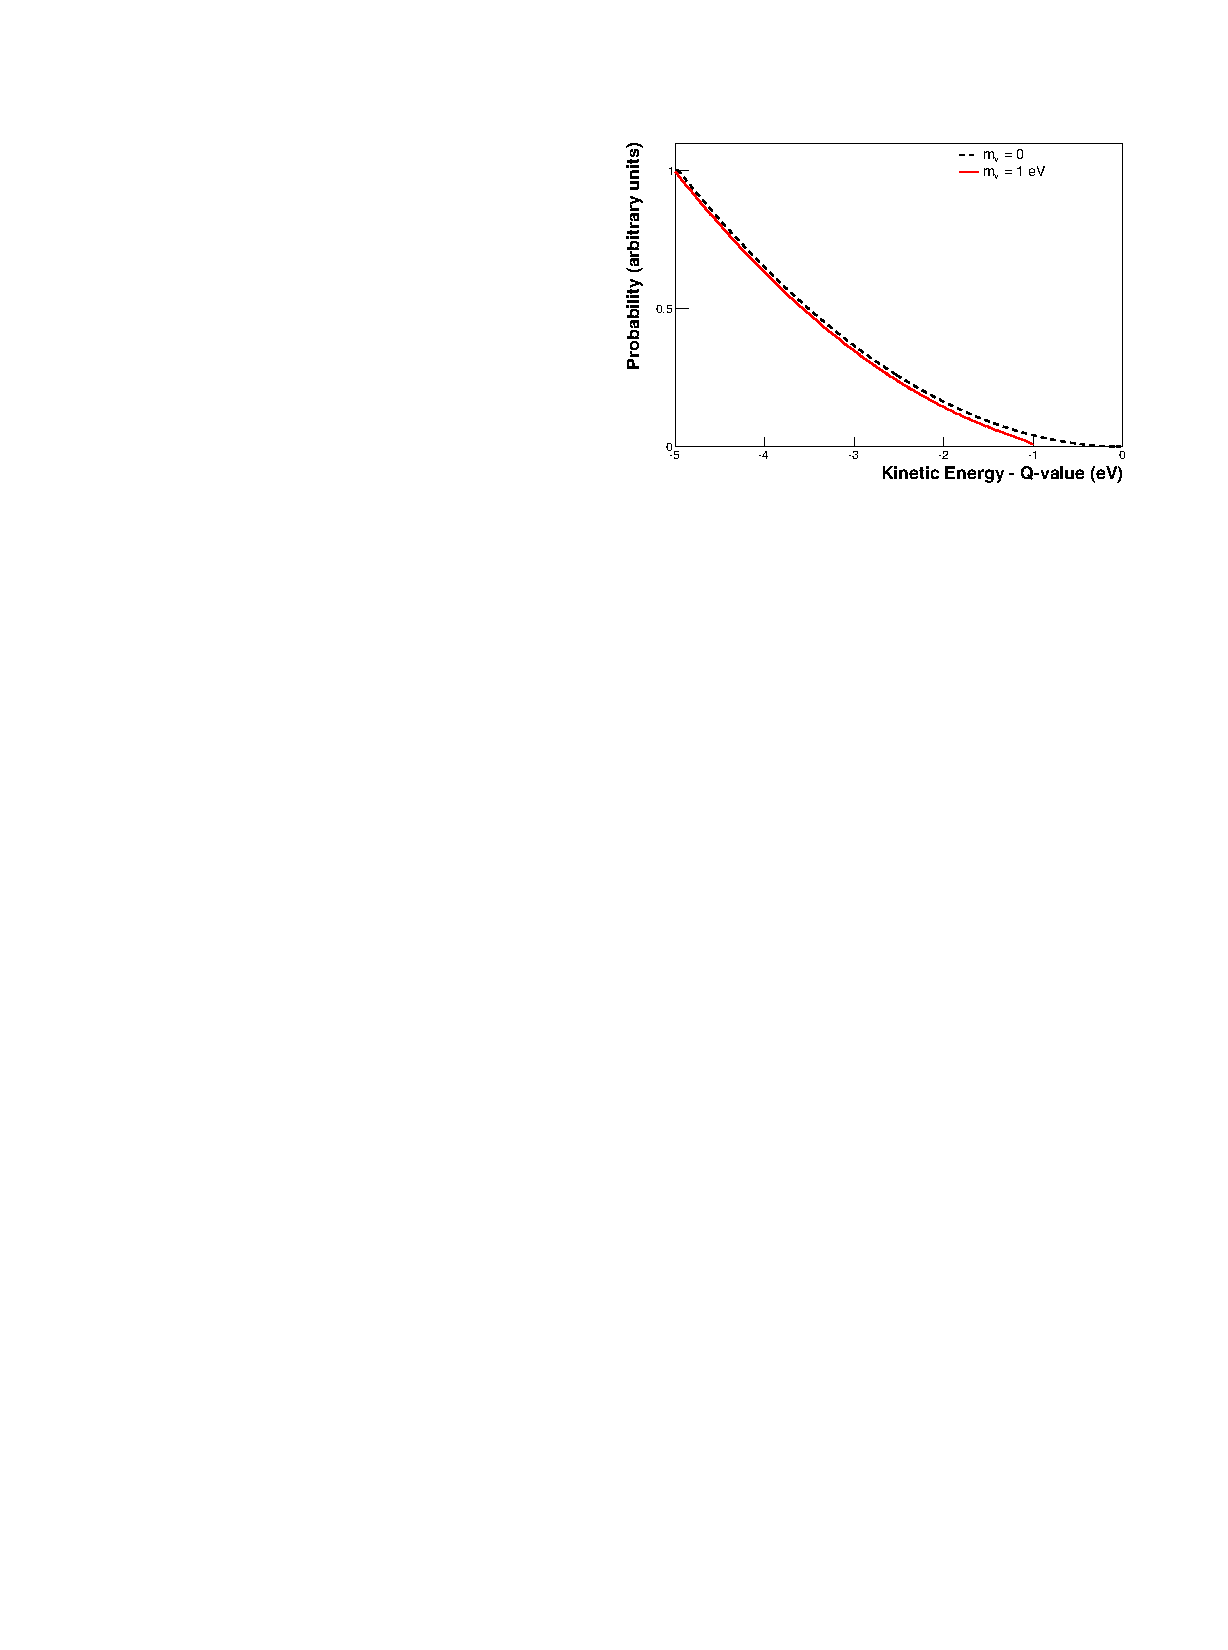
\includegraphics[width=0.5\textwidth]{Neutrinos/BetaDecay}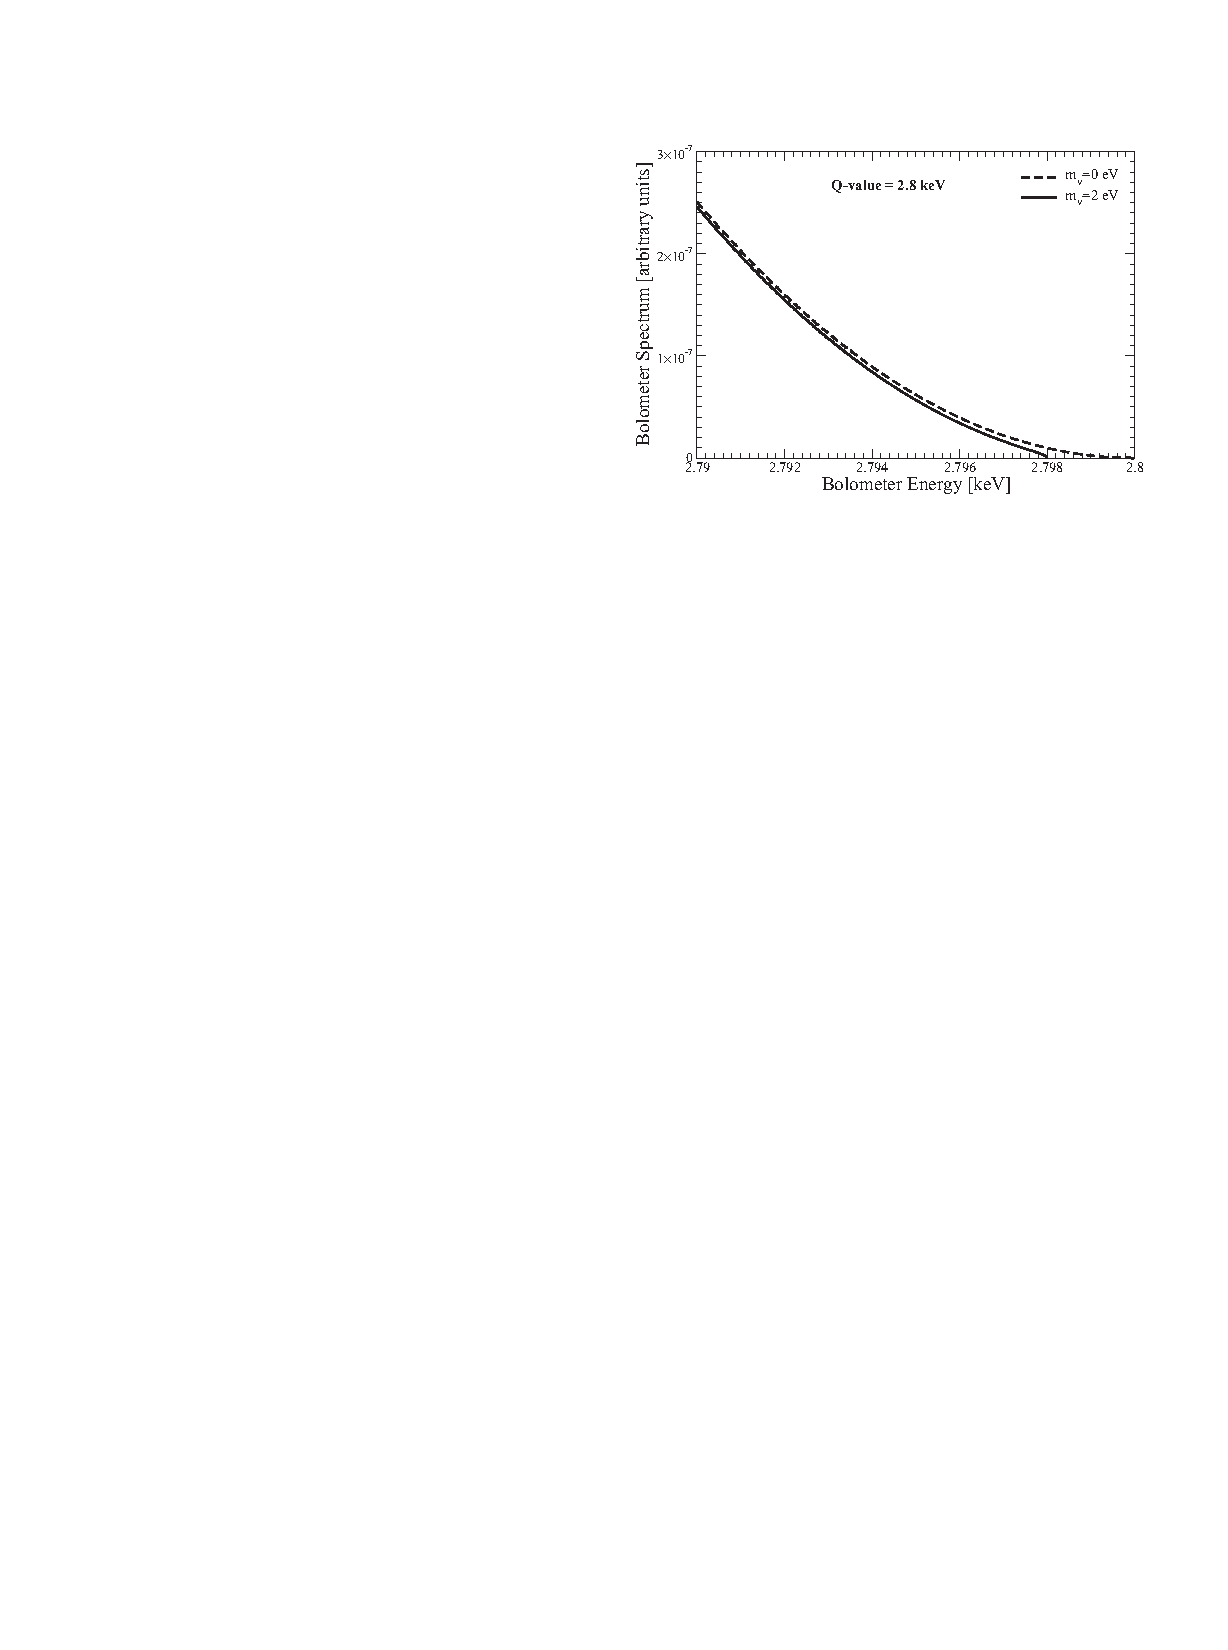
\includegraphics[width=0.5\textwidth]{Neutrinos/e-capture}
\caption{Shown on the left is the kinematic suppression of the
  $\beta$-decay spectrum in the presence of a zero or 1\,eV $\beta$-decay
  neutrino mass. On the right are the bolometer spectra for endpoint
  energies in electron capture for effective zero and 2\,eV neutrino
  masses.}
\label{fig:kinematic_mass}
\end{figure}

Current kinematic measurements from Mainz~\cite{Kraus:2004zw} and Troitsk~\cite{Aseev:2011dq} limit the electron antineutrino mass to $< 2.0$~eV. The KATRIN experiment~\cite{Angrik:2005ep} will begin taking data in 2016 and is expected to improve this limit by a factor of ten. 

Within the standard neutrino mass and cosmological paradigm, the kinematic and cosmological measurements of the neutrino mass are connected through the PMNS matrix. Thus, the combination of cosmological and terrestrial neutrino mass measurements tests our cosmological neutrino model. A discrepancy could point to new physics (e.g. modified thermal history through neutrino decay).

Improving kinematic measurements beyond KATRIN's $0.2$~eV limit will require new technology since KATRIN will be limited by the final state spectrum of the source itself, specifically rotational-vibrational states of molecular Tritium. One of the new approaches is a calorimetric measurement of the electron-capture spectrum of $^{163}$Ho. The calorimetric measurement of the $^{163}$Ho endpoint is insensitive to the details of the source configuration and may provide an avenue for eventually surpassing the KATRIN sensitivity. Interestingly, upcoming experiments such as ECHO~\cite{Eliseev:2015pda}, HOLMES \cite{Ceriale:2015mtn}, and NuMECS~\cite{Croce:2015kwa} utilize multiplexed superconducting detectors, the same technology baselined for the CMB-S4 experiment. Another promising direction for direct neutrino mass measurement is the frequency-based technique employed by the Project-8 experiment~\cite{Asner:2014cwa}. Project-8 aims to measure the beta-decay spectrum of Tritium by measuring the frequency of cyclotron radiation emitted by the decay electrons when trapped in a magnetic field. An exciting aspect to this frequency-based technique is the potential to trap atomic Tritium which is not subject to the rotational-vibrational excitations of molecular Tritium. A spectroscopic measurement using atomic Tritium could eventually achieve sensitivities of $<0.04$~eV, a level comparable to cosmological measurements.

%Direct mass measurement from tritium decay works on the following premise.  The $\beta$-decay for tritium produces Helium-3 and an electron and anti-neutrino that carry 18.6 keV of energy between them.  While in most decays this energy is distributed evenly neutrino and electron, there are rare decays where most of the energy is carried by the electron.  If the lightest neutrino is massless, the electron energy may be arbitrarily close to 18.6 eV.  However, for a non-zero mass for the lightest neutrino there is necessary a gap in the electron energy spectrum.  A careful measurement of the electron energy spectrum can therefore constrain the mass of the lightest neutrino.

\subsection{Lepton number violation: Majorana vs. Dirac neutrinos}
One of the more interesting connections between cosmological measurements of neutrino mass and terrestrial experiments is the complementarity between cosmological neutrino mass measurements and the search for neutrinoless double beta decay (NLDBD). NLDBD is a hypothetical decay mode of certain nuclei where two neutrons convert to two protons and two electrons with no emission of neutrinos. The observation of NLDBD would be transformational demonstrating that neutrinos are Majorana particles and revealing a new lepton-number-violating mechanism for mass generation. This new physics could potentially explain both the smallness of neutrino masses and matter-antimatter asymmetry in the universe.

Initial results from the current generation of NLDBD searches limit the NLDBD half life, $T^{0\nu}_{1/2}$, to be larger than  $\sim2\times10^{25}$~years~\cite{Agostini:2013mzu,Auger:2012ar,Artusa:2014lgv}.%\cite{Gerda, Exo, Cuore}.
 The full sensitivity of these experiments is expected to be in the range of $10^{25}-10^{26}$~years~\cite{Geesaman:2015fha}. Planning and technology development is already underway for next generation ``ton-scale'' NLDBD searches which would achieve sensitivities of $10^{27}-10^{28}$~years~\cite{Geesaman:2015fha}.

We can illustrate the connection between NLDBD searches to cosmological determinations of neutrino mass by examining the simplest case where NLDBD is mediated by exchange of light Majorana neutrinos. Within the context of this mechanism, we can define an ``effective neutrino mass,'' $m_{\beta\beta}$, given by 

\beq
m_{\beta\beta}^{2} = ( \sum_i U_{ei}^{2}m_{\nu i} )^{2}
\label{eq:mbb}
\eeq
where $m_{\nu i}$ are the light neutrino masses and $U_{ei}$ is the usual PMNS mixing matrix including two unknown Majorana phases. The NLDBD half-life is then given by 

\beq
(T^{0\nu}_{1/2})^{-1} = G^{0\nu}\cdot (M^{0\nu} )^{2}\cdot m_{\beta\beta}^2,
\eeq

where $G^{0\nu}$ is a phase space integral and $M^{0\nu}$ is the nuclear matrix element. In this simple scenario, the signal from NLDBD experiments can be directly related to other measures of neutrino mass. Figure~\ref{fig:NLDBD} illustrates this relationship between the effective neutrino mass and the lightest neutrino mass including limits and sensitivities of current and next generation NLDBD searches.

\begin{figure}[h!]
\centering 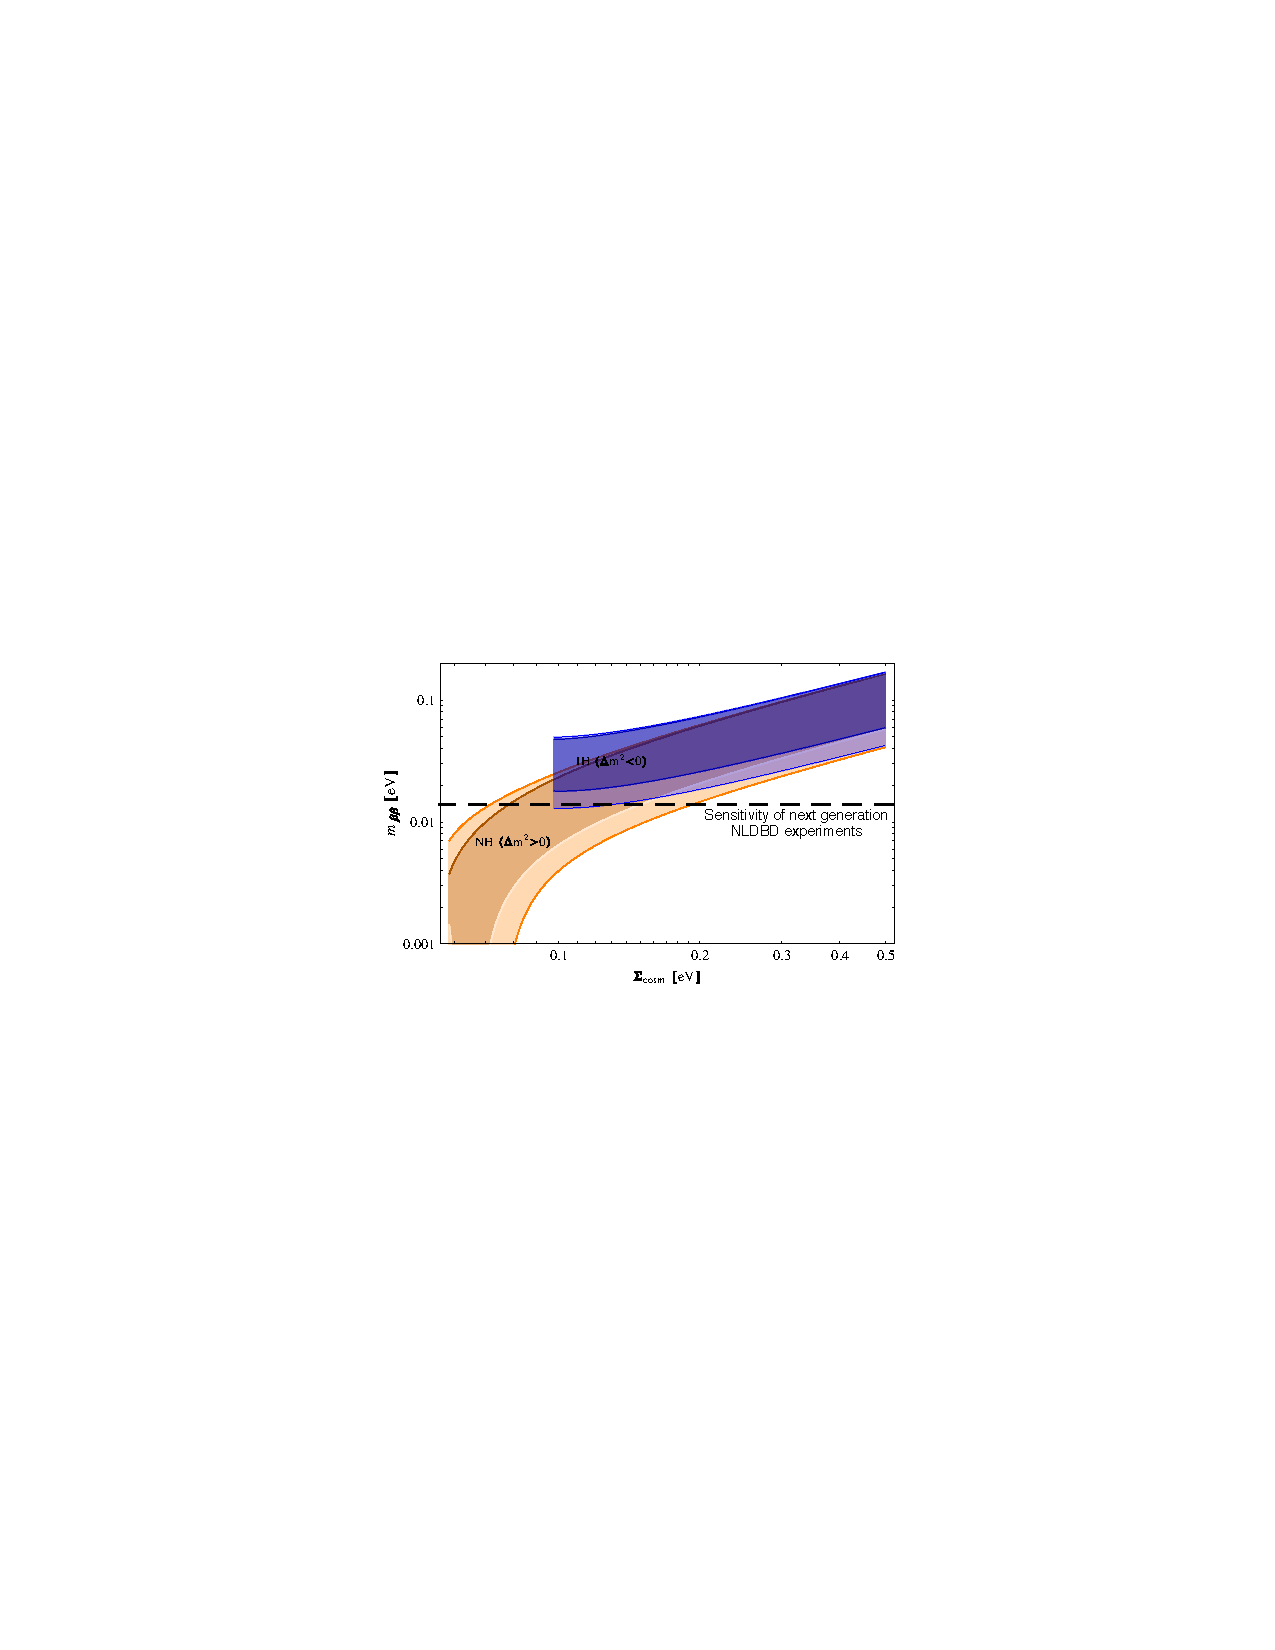
\includegraphics[width=0.8\textwidth]{Neutrinos/mbb_v_sum_m_nu.pdf}
\caption{Plot of effective neutrino mass versus $\sum m_\nu$ in the scenario where NLDBD is mediated by light neutrino exchange. The blue band corresponds to inverted ordering and the orange band corresponds to normal ordering. Next generation ``ton-scale'' NLDBD searches will have sensitivities down to $m_{\beta\beta}>15$~meV (dashed line). Figure from~\cite{Dell'Oro:2014yca}}
\label{fig:NLDBD}
\end{figure}

The complementarity between cosmological neutrino mass measurement and NLDBD can be understood by considering scenarios where NLDBD experiments either observe or fail to observe NLDBD. In the absence of a signal in next generation NLDBD searches, a cosmological measurement constraining $\sum m_\nu > 100$~meV (corresponding to either the inverted hierarchy or a minimum neutrino mass of 50~meV) would strongly point to neutrinos being Dirac particles (see Fig.~\ref{fig:NLDBD}). On the other hand, if NLDBD is observed, equation~\ref{eq:mbb} shows that cosmological measurements of $\sum m_\nu$ are sensitive to the Majorana phases. For example, Fig.~\ref{fig:MajoranaPhase} shows that in the inverted mass hierarchy cosmological measurements together with NLDBD measurements can constrain one of the Majorana phases. Perhaps even more interesting would be the situation where cosmological and NLDBD measurements violate equation~\ref{eq:mbb} indicating new physics beyond the simple model of light Majorana neutrino mediated decay.

\begin{figure}[h!]
\centering 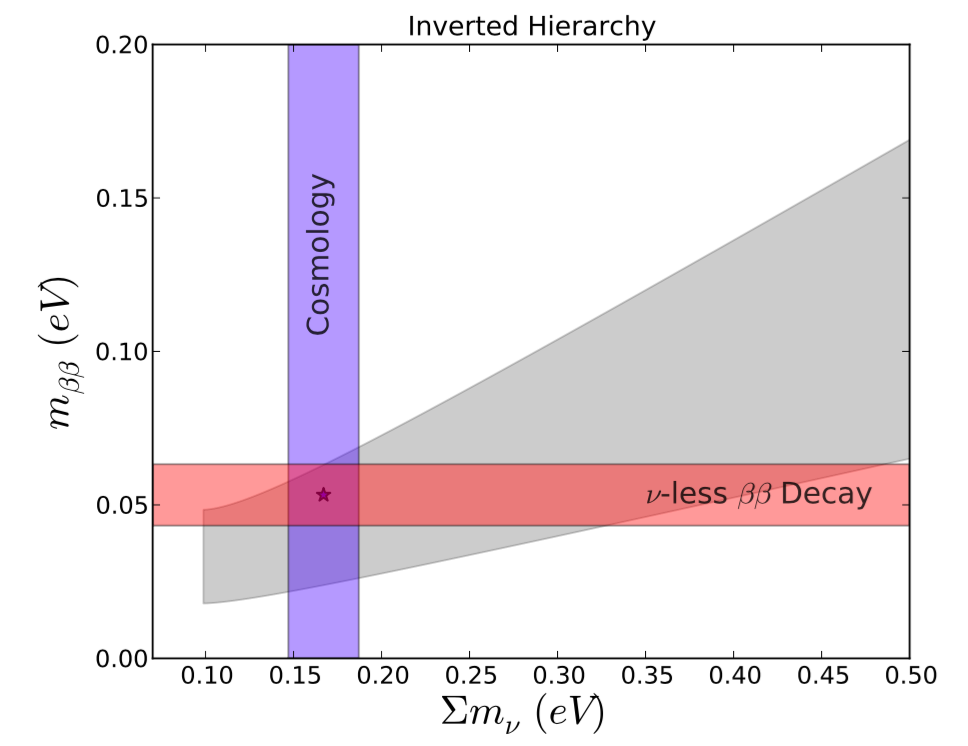
\includegraphics[width=0.70\textwidth]{Neutrinos/IH_MajoranaPhase.png}
\caption{Relationship between effective neutrino mass as measured by NLDBD experiments versus $\sum_i m_{\nu i}$ as measured by cosmology for the inverted hierarchy. The gray band corresponds to a region allowed by existing measurements where the width of the band is determined by the unknown Majorana phase. }
\label{fig:MajoranaPhase}
\end{figure}


%In addition to the effort to constraint the sum of the neutrino masses from cosmology, a variety of lab-based experiments are constraining the angles, phases and masses describing neutrino mixing.  While cosmology is insensitive to mixing angles, 

\subsection{Neutrino mass ordering and CP violation}
In the case of normal ordering with non-degenerate neutrino mass, the CMB-S4 measurement of $\sum m_\nu$ will provide a 2--4$\sigma$ determination of the neutrino mass ordering. Fully characterizing neutrino mass ordering and CP violation is one of the goals of the terrestrial neutrino physics program~\cite{Patterson:2015xja}. The upcoming reactor neutrino experiment JUNO~\cite{An:2015jdp} is scheduled to start data taking around $\sim$ 2020 and will have $\sim$ 2--3$\sigma$ sensitivity to neutrino ordering after six-years of operation. Future experiments measuring atmospheric neutrino oscillations (e.g Hyper-K~\cite{Abe:2015zbg}, DUNE~\cite{Goodman:2015gmv}, KM3NeT/ORCA~\cite{Adrian-Martinez:2016fdl}) can also resolve the neutrino mass ordering. For example, KM3NeT/ORCA forecasts a 3$\sigma$ measurement of the mass ordering by around 2023. Accelerator neutrino experiments are the only known method for exploring neutrino CP violation and in some cases, are also sensitive to neutrino mass ordering. In a $\sim 5$-year timescale, the currently operating NO$\nu$A experiment~\cite{Adamson:2016tbq} may determine the neutrino ordering at the 2--3$\sigma$ level, provided that $\delta_{CP}$ falls into a favorable range. Hyper-K will measureme $\delta_{CP}$, though it requires external input regarding the neutrino ordering (e.g. from Hyper-K atmospheric neutrinos or from cosmology). The next-generation US-based long-baseline neutrino-oscillation experiment, DUNE, is planned to start operation around 2024, and will measure both the neutrino mass ordering (at the 2--4$\sigma$ level) and $\delta_{CP}$. External input on neutrino ordering from other sources such as CMB-S4 would provide a strong consistency check of DUNE results and test the three-neutrino paradigm.

In the scenario where the neutrino mass specrtum is normally ordered and non-degenerate, CMB-S4 would be a strong complement to terrestrial experiments by providing a measurement of neutrino ordering that is independent of oscillation parameters and $\delta_{CP}$. Under all circumstances, the combination of CMB-S4 with terrestrial determinations of neutrino ordering will provide a definitive measurement of the neutrino mass spectrum.


%The relation between cosmological measurement from CMB-S4, kinematic constraints constraints expected from KATRIN~\cite{Angrik:2005ep}, and upcoming long-baseline oscillation experiments is shown in Fig.~\ref{fig:neutrino-noose}. The three approaches to neutrino mass and mixing are complementary and the combination of their results will either reveal new physics in the neutrino sector or provide a definitive measure of the full neutrino mass spectrum. 

%The mass of the lightest neutrino is clearly related to the sum of the masses but the lower bound for the sum does not exist for the lightest neutrino.  In this sense the two approaches are complimentary as they cover different aspects of the neutrino mass hierarchy.

\begin{figure}[h!]
\centering 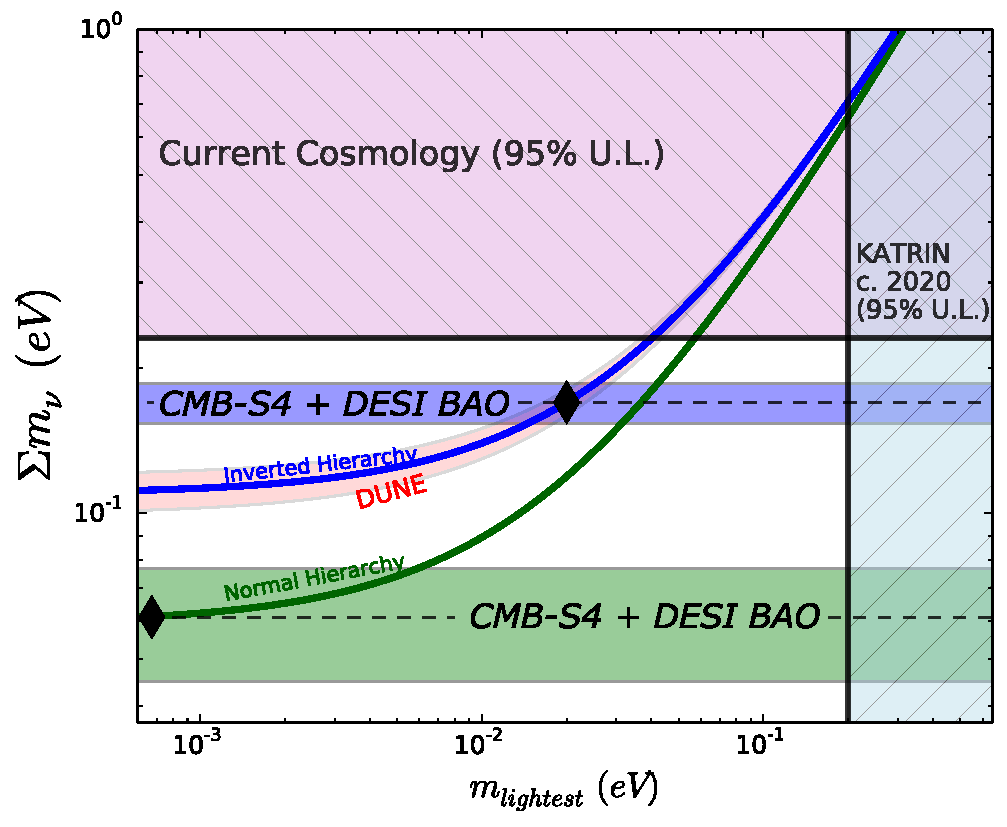
\includegraphics[width=0.55\textwidth]{Neutrinos/numass_combine_dune}
\caption{Shown are the current constraints and forecast sensitivity of
  cosmology to the neutrino mass in relation to the neutrino mass
  hierarchy.  In the case of an ``inverted ordering,'' with an
  example case marked as a diamond in the upper curve, the CMB-S4 (with DESI BAO prior)
  cosmological constraints would have a very high-significance
  detection, with $1\sigma$ error shown as a blue band.  In the case
  of a normal neutrino mass ordering with an example case marked as
  diamond on the lower curve, CMB-S4 would detect the lowest
  $\sum m_\nu$ at $\gtrsim 3 \sigma$. Also shown is the
  sensitivity from the long baseline neutrino experiment (DUNE) as the
  pink shaded band, which should be sensitive to the neutrino
  hierarchy. Figure adapted from the Snowmass CF5 Neutrino planning document.
 }
\label{fig:neutrino-noose}
\end{figure}


\subsection{Sterile Neutrinos}
\label{sec:sterile_neutrinos}

Mechanisms of introducing neutrino mass often include sterile
neutrinos, with both Majorana and Dirac terms potentially
contributing (e.g., Ref.~\cite{Langacker:2011bi}):
\bea
\mathcal{L}_D &=& -m_D\left(\bar\nu_L\nu_R + \bar\nu_R\nu_L\right) \\
\mathcal{L}_M &=& -\frac{1}{2}m_T\left(\bar\nu_L\nu_L^c + \bar\nu_L^c\nu_L\right) 
-\frac{1}{2}m_S\left(\bar\nu_R\nu_R^c +\bar\nu_R^c\nu_R\right) =
-\frac{1}{2}m_T\left(\bar\nu_a\nu_a\right) -\frac{1}{2}m_S\left(\bar\nu_s\nu_s\right),
\eea
where $\nu_a \equiv \nu_L + (\nu_L)^c$ and $\nu_S \equiv \nu_R +
(\nu_R)^c$ are active and sterile Majorana two component spinors,
respectively. The mass $m_T$ can be generated by a Higgs triplet,
i.e., $m_T = y_T\langle \phi^0_T\rangle$, or from a higher-dimensional
operator involving two Higgs doublets with coefficients
$C/\mathcal{M}$. For dimension 5 operators, this becomes the Type-I
seesaw mechanism, where both Majorana and Dirac terms are present and
$m_S \gg m_D$.


A number of recent neutrino oscillation experiments have reported anomalies
that are possible indications of four or more neutrino mass eigenstates. The
first set of anomalies arose in short baseline oscillation experiments.
First, the Liquid Scintillator Neutirno Detector (LSND) experiment observed
electron antineutrinos in a pure muon antineutrino
beam \cite{Athanassopoulos:1997pv}. The MiniBooNE Experiment also observed
an excess of electron neutrinos and antineutrinos in their muon
neutrino beam \cite{Aguilar-Arevalo:2013pmq}. Two-neutrino oscillation
interpretations of these results indicate mass splittings of $\Delta m^2
\approx 1\rm\ eV^2$ and mixing angles of $\sin^2 2\theta \approx
3\times 10^{-3}$ \cite{Aguilar-Arevalo:2013pmq}. Another anomaly
arose from re-evaluations of reactor antineutrino fluxes that
indicate an increased flux of antineutrinos as well as a lower
neutron lifetime and commensurately increased the antineutrino events
from nuclear reactors by 6\%. This caused previous agreement of
reactor antineutrino experiments to have a $\approx$6\% deficit
\cite{Mention:2011rk,Huber:2011wv}. Another indication consistent with
sterile neutrinos was observed in radio-chemical gallium experiments for solar
neutrinos. In their calibrations, a 5-20\% deficit of the measured
count rate was found when intense sources of electron neutrinos from
electron capture nuclei were placed in proximity to the
detectors. Such a deficit could be produced by a $m_S >1\rm\ eV$ sterile
neutrino with appreciable mixing with electron neutrinos
\cite{Bahcall:1994bq,Giunti:2010zu}. Some simultaneous fits to the
short baseline anomalies and reactor neutrino deficits, commensurate
with short baseline constraints, appear to prefer at least two extra
sterile neutrino states \cite{Conrad:2012qt,Kopp:2013vaa}, but see~\cite{Giunti:2015mwa}. Because such neutrinos have relatively
large mixing angles, they would be thermalized in the early universe
with a standard thermal history, and affect primordial nucleosynthesis
\cite{Abazajian:2002bj} and CMB measurements of $\Neff$.  These implications will be discussed in the next chapter.

To accomodate $m_S = \mathcal{O}({\rm eV})$ with some mixing between active
and sterile states in the neutrino mass generation mechanism discussed
above requires mixing between active and sterile states with the same
chirality, which does not occur for pure Majorana or Dirac mass cases
or for the conventional seesaw mechanism. One proposed mechanism is
the minimal mini-seesaw ($m_T =0$ and $m_D\ll
m_S\sim\mathcal{O}(\mathrm{eV})$,
e.g. Ref.\cite{deGouvea:2011zz,Donini:2012tt} ). In such models, the
sterile neutrinos can have the appropriate masses and mixings to
accommodate the short baseline anomalies. For standard thermal
histories, these sterile neutrinos are typically fully thermalized
\cite{Abazajian:2002bj}. However, it is possible they are partially
thermalized in two extra neutrino models \cite{Jacques:2013xr}.

Interestingly, there are combinations of CMB plus LSS
datasets that are in tension, particularly with a smaller amplitude of
fluctuations at small scale than that inferred in zero neutrino mass
models. This would be alleviated with the
presence of massive neutrinos, extra neutrinos, or both. In particular,
cluster abundance analyses \cite{Wyman:2013lza,Ade:2015fva} and weak lensing analyses
\cite{Battye:2013xqa} indicate a lower amplitude of
fluctuations than zero neutrino mass \cite{Giusarma:2014zza}. Baryon Acoustic
Oscillation measures of expansion history are affected by the presence
of massive neutrinos, and nonzero neutrino mass may be indicated 
\cite{Beutler:2014yhv}, though 2015 Planck results show a lack of such
alleviation in cases with massive or extra neutrinos
\cite{Ade:2015xua}. 

There is a potential emergence of both laboratory and cosmological
indications of massive and, potentially, extra neutrinos. However, the
combined requirements of the specific masses to produce the short
baseline results, along with mixing angles that require thermalized
sterile neutrino states, are inconsistent at this point with
cosmological tension data sets
\cite{Joudaki:2012uk,Archidiacono:2013xxa}. The tension data sets are
not highly significant at this point ($\lesssim 3\sigma$), and there
are a significant set of proposals for short baseline oscillation
experiment follow up \cite{Abazajian:2012ys}. 

%Future high-sensitivity
%probes of neutrino mass and number such as CMB-S4 will be able to
%definitively test for the presence of extra neutrino number and mass
%consistent with sterile neutrinos.

In fact, we know little about the sterile neutrino sector, though its possible existence is in part motivated by the experimental establishment that neutrinos have nonzero rest masses as discussed above. CMB-S4 could shed light on the sterile neutrino mass and vacuum flavor mixing parameters invoked to explain the experimental neutrino anomalies. It must be kept in mind that sterile neutrinos might have different masses and much smaller vacuum mixing with active neutrinos species. Telltale signatures in $\Neff$, $\sum m_{\nu}$, and $Y_p$ can allow CMB-S4 to probe this larger parameter space.  These measurements will be discussed in the next chapter.



\section{Detection Scenarios for Neutrino Physics} \label{sec:neuscenarios}

As discussed in Section~\ref{sec:lab}, the measurements of the absolute scale of the neutrinos masses from the lab and from cosmology are complimentary in that they are sensitive to different parameters.  In principle, there are a variety of possible scenarios where detections are made both in cosmology and in the lab.  However, given current constraints, most scenarios that involve mostly conventional neutrino physics will result in upper limits from the lab based measurements and a detection of $\sum m_\nu$ and/or $\Delta\Neff \equiv \Neff - 3.046$.  We will discuss $\Neff$ is greater detail in the next chapter but here it serves as a measurement of the total number of thermal neutrinos which calibrates the cosmological mass measurement. A plausible list of detection scenarios are shown in Table~\ref{table:neutrinoscenarios}:

\begin{itemize}
\item Conventional neutrino mass scenarios imply majorana masses with a normal or inverted hierarchy.  The normal hierarchy with $\sum m_\nu \simeq 58$~meV is perhaps the most conventional as it reflects the same hierarchical / non-degenerate masses that appear in the charged fermions of the Standard Model.  This scenario is only detectable in the near term via cosmology due to the small size of the neutrino masses.  Somewhat more exotic is the case of a Dirac mass, as it predicts the existence of new light states.

\item The more exotic possibility is that there could be sterile neutrinos that are consistent with a variety of anomalies, as discussed in Section~\ref{sec:sterile_neutrinos}.  In this case, we would observe a correlated signature in both a excess in $\sum m_\nu$ and $\Delta \Neff$ due to the presence of thermalized sterile neutrinos in addition to the active neutrinos.  The sterile neutrino parameters that are most consistent with the anomalies in short-baseline experiments are already in tension with cosmology but would be detected at high significance if these models describe our universe.  

\item Given the current cosmological constraints on $\sum m_\nu$, detections of $m_\beta$ and $m_{\beta \beta}$ in near term experiments would require a significant change to the thermal history.  In particular, a detection of a Majorona mass at the $0.25 \, {\rm eV}$ level would predict a $\sum m_\nu$ that is already excluded by cosmology.  Making the current (or future) limit consistent then requires a mechanism that satisfies both the present bound on $\sum m_\nu$ and the current constraints on $\Neff$.


\item There are a variety of scenarios that produce $\Delta \Neff  \gtrless 0$ without changing neutrino physics.  In this case, the neutrino physics may follow a conventional pattern like the normal hierarchy.  In principle, one would distinguish scenarios where there is no change to the number density of neutrinos (dark radiation) from scenarios where the neutrinos are diluted or enhanced by a change to the thermal history (late decay) as the interpretation of $\sum m_\nu$ depends on the neutrino number density.  However, given that current measurements allow for $< 10$ percent change to the neutrino number density, we would need to detect $\sum m_\nu$ at 10$\sigma$ to be sensitive to such a change.  Nevertheless, dark radiation and changes to the thermal history can make correlated predictions for other experiments as we will discuss in the next Chapter.

\item The neutrino sector may be rich in new physics and CMB Stage IV provides us with significant new discovery potential. Finding evidence for sterile neutrinos or a primordial lepton number larger than the baryon number, but well below the present BBN bound, $\sim 0.1$, would be a signal event for particle physics. Sterile neutrinos with masses of order $\sim 1\,{\rm eV}$ and relatively large vacuum mixing with active species ($\sin^2 \theta \sim 10^{-3}$), like those invoked to explain the neutrino anomalies, would have relic densities and relic energy spectra comparable to those of the active neutrinos and therefore are easy targets for CMB constraint or detection as discussed above. However, a primordial lepton number $> {10}^{-4}$ would suppress the production of these sterile neutrinos in the early universe. Moreover, sterile neutrinos with tiny vacuum mixing could escape laboratory detection, yet still might acquire small but significant population in the early universe through lepton number-induced resonant conversion of active neutrinos~\cite{Abazajian:2005gj}. Both of these cases could leave telltale signatures in CMB observables, specifically in $\Neff$, $\sum m_\nu$, and $Y_p$. The pattern of changes in these observables, compared to results from high precision neutrino transport and flavor oscillation physics coupled to weak and nuclear reactions, can give distinctive markers for sterile neutrino mixing physics (see e.g. \cite{Smith:2006uw, Grohs:2015tfy}).

\end{itemize}
\begin{table}[t!]
\begin{center}
\begin{tabular}
{| l | c c c c | p{5cm} | }\hline Scenario & $m_{\beta \beta}$ & $m_{\beta}$&  $\sum m_\nu$ & $\Delta \Neff$ & Conclusion \\
\hline 
Normal hierarchy & $< 2\sigma$ & $< 2\sigma$  & $60 \, {\rm meV}$ & 0 & Normal neutrino physics; no evidence for BSM
\\[.2cm]
Dirac Neutrinos & $< 2\sigma$ & $< 2\sigma$  & $350  \, {\rm meV}$ & 0 & Neutrino is a dirac particle \\[.2cm]
Sterile Neutrino & $< 2\sigma$ & $< 2\sigma$   & $350  \, {\rm meV}$ & $>0$ & Detection of sterile neutrino consistent with short-baseline \\
\hline
Diluted Neutrinos & $ 0.25 \, {\rm eV}$ & $ 0.25 \, {\rm eV}$  & $<150  \, {\rm meV}$ & $< 0$ & Modified thermal history (e.g. late decay) \\[.2cm]
Exotic Neutrinos & $ 0.25 \, {\rm eV}$ & $ 0.25 \, {\rm eV}$  & $<150  \, {\rm meV}$ & $0$ & e.g. Modified thermal history; (e.g. neutrino decay to new particle) \\[.2cm]
Excluded & $ 0.25 \, {\rm eV}$ & $ 0.25 \, {\rm eV}$  & $500  \, {\rm meV}$ & $0$ & Already excluded by cosmology \\
\hline
Dark Radiation & $< 2\sigma$ & $< 2\sigma$  & $60  \, {\rm meV}$ & $>0$ & Evidence for new light particles; normal hierarchy for neutrinos
\\[.2cm]
Late Decay & $< 2\sigma$ & $< 2\sigma$  & $60  \, {\rm meV}$ & $<0$ & Energy-injection into photons at temperature $T \lesssim 1$ MeV \\
\hline 
\end{tabular}
\caption{Relation between neutrino experiments and cosmology.  We include the measurement of the Majorona mass via NLDBD ($m_{\beta \beta}$) or a kinematic endpoint ($m_\beta$) compared to the cosmological measurement of the sum of the masses $\sum m_\nu$ and the CMB measurement of $\Neff$.  Here $< 2 \sigma$ indicates an upper limit from future observations.  For Section~\ref{sec:lab}, one can use $\sigma(m_{\beta\beta}) \approx 0.075 \, {\rm eV} $ and $\sigma(m_\beta) \approx 0.1 \, {\rm eV} $ for observations on the timescale of CMB-Stage IV.  For $\Delta\Neff$ the use of $\gtrless 0$ indicates a significant deviation from the Standard Model value.}
\label{table:neutrinoscenarios}
\end{center}
\end{table} 


%Neutrinoless double beta decay can occur in a variety of nuclei if neutrinos have a non-zero Majorana mass but does not occur for a Dirac mass.  The decay is effectively involves two neutrons decaying to two protons and two electrons with no associated neutrinos.  The flavor structure of this decay means the amplitude is proportional to $|m_{ee}|^2$ where $m_{ee} = \sum_i m_i U_{ei}$, $U$ is the PMNS matrix, and $m_i$ are the mass eigenstates.  While cosmology can not directly determine whether the mass is Majorana or Dirac, a detection of such a decay could establish that it it has a Majorana mass.  Also, like tritium decay, there is no required lower limit on $m_{ee}$ and therefore there is no level of sensitivity that would guarantee a detection.

% Possible anomalies found in short baseline oscillation experiments (LSND~\cite{Aguilar:2001ty},
% MiniBooNE~\cite{AguilarArevalo:2010wv}, etc.) may be explained as an active-sterile neutrino
% oscillation.  Parameters required to these fits typically lead to
% thermalization of the sterile species in the early universe before
% neutrino decoupling, resulting in non-standard $N_\mathrm{eff}$ and
% contribution to $\sum m_\nu$.  Further description can be found
% below in Section~\ref{sec:sterile_neutrinos}.

%[AK:6/3] The mass hierarchy may be determined by terrestrial experiments
%as well.  NO$\nu$A experiment can determine the hierarchy at
%2--3$\sigma$ level if the $CP$-violating phase $\delta_{CP}$ falls into
%the favorable range of around $3\pi/2$ ($\pi/2$) for normal (inverted)
%hierarchy in a $\sim 5$-year timescale [1].  Possible ambiguity arises
%if the nature chooses unfavorable $\delta_{CP}$; this can be resolved by
%a future measurement of $\delta_{CP}$ by a next-generation long-baseline
%experiment such as Hyper-Kamiokande.  [AK: was there a US competitor of
%Hyper-K?  Is it LBNF?]
%
%The next-generation US-based long-baseline neutrino-oscillation
%experiment, LBNF, is planned to start operation around 2024.
%LBNF would resolve the hierarchy at 2--4$\sigma$ level depending on the
%$\delta_{CP}$ [2].
%
% China-based next-generation reactor neutrino experiment, JUNO, is also
% sensitive to the mass hierarchy.  It is scheduled to start data taking
% around $\sim$ 2020 and will have $\sim$ 2 (3?)$\sigma$ sensitivity to
% resolve the hierarchy after a six-year operation [3].  [AK: I have not
% understood what they mean by ``crossing sensitivity.'']
%
% Atmospheric neutrino oscillation can also be used to resolve mass
% hierarchy [4,5].  KM3NeT/ORCA forecasts to resolve the mass hierarchy at
% a 3$\sigma$ level by around 2023.
%
% [AK: I have collected schedule information from slides etc., but we may
% query PIs of each experiment to get firm citation.]

%Cosmological measurements and these terrestrial hierarchy measurements
%are complementary to each other.  For example, if cosmology measures the sum of
%the neutrino mass heavier than $\sim 116$\,meV, the terrestrial
%experiments are the only way to determine the hierarchy.  In turn,
%in this case of $\sum m_\nu > 116$\,meV,
%determination of the hierarchy by terrestrial experiments would allow
%cosmology to constrain the mass of the lightest neutrino without
%discrete ambiguity.
%In a similar manner to the cosmology being dependent on the central
%value of $\sum m_\nu$, 
%long-baseline oscillation experiments would suffer from
%relatively low sensitivity to the hierarchy
%if the $\delta_{CP}$ turns out to be unfavorable.
%Also, it is worth noting that all the terrestrial experiments use matter
%effect to resolve the hierarchy.  Some of the beyond-the-standard models
%involve modification of the neutrino interaction and thus that of the
%matter
%effect [citation needed].  Cosmological measurements, on the other hand, 
%are relatively
%insensitive to possible modification of interaction.  Consistency check
%between the terrestrial measurements and cosmological constraints would
%probe BSM physics in neutrino interaction.

%[1] https://doi.org/10.1146/annurev-nucl-102014-021916
%[2] https://arxiv.org/abs/1601.05471
%[3] https://arxiv.org/abs/1507.05613
%[4] http://arxiv.org/abs/1401.2046
%[5] http://arxiv.org/abs/1601.07459


%%
%% Populate the .bib file with entries from SPIRES Bibtex (preferred)
%% or ADS Bibtex (if no SPIRES entry).
%%  SPIRES will also supply the CITATION line information; please include it.
%%


